\documentclass[a4paper,12pt,oneside]{report}
\usepackage[utf8]{inputenc}
\usepackage{graphicx}
\usepackage{caption} % For customizing captions
\usepackage{subcaption} % For subfigures
\usepackage{amsmath}
\usepackage{amsthm}
\usepackage{amsfonts}
\usepackage{textpos}
\usepackage{amssymb}
\usepackage{float}
\usepackage{multirow}
\usepackage{booktabs}
\usepackage[ruled, noline, linesnumberedhidden, shortend]{algorithm2e}
\usepackage[hyphens]{url}

\newtheoremstyle{named}{\topsep}{\topsep}{\itshape}{0pt}{\bfseries}{\vspace{\baselineskip}}{\newline}{\thmnote{#3}}
\theoremstyle{named}
\newtheorem{named}{Theorem}[section]

\usepackage[labelfont=bf]{caption}
\usepackage{hyperref}

\graphicspath{{images/}}

\setlength{\voffset}{-0.5in}
\setlength{\headsep}{5pt}

\title{A Frank-Wolfe Algorithm for Grid-free Reconstruction of Dirac Impulses}
\author{David Rochinha Chaves}

\def\maketitle{
\newlength{\drop}
\newlength{\tpheight}\setlength{\tpheight}{0.9\textheight}
\newlength{\txtheight}\setlength{\txtheight}{0.9\tpheight}
\begingroup
\thispagestyle{empty}
\drop=0.1\txtheight
\begin{textblock*}{4in}[0.3066,0.39](0.in,0.in)
    
\includegraphics[width=2.9in]{EPFLlogo}
\end{textblock*}
\begin{textblock*}{4in}[0.3066,0.39](5.in,-0.1in)
    
\includegraphics[width=2.2in]{LABlogo}
\end{textblock*}
\vspace{1.5in}
\centering 
{\Large \rmfamily École Polytechnique Fédérale de Lausanne}\\[2\baselineskip]
{\Large \textbf{\textrm{Master Thesis}}}\\
[3\baselineskip]
{\LARGE \textbf{\textsf{A Frank-Wolfe Algorithm for Grid-free Reconstruction of Dirac Impulses}}}\\[1\baselineskip] 
\large \textsf{by David Rochinha Chaves}\\
[2.5\baselineskip]
\textit{Supervisor} \\
Adrian Jarret \\
[1\baselineskip]
\textit{Advisor} \\
Prof. Martin Vetterli\\
[2\baselineskip]
\centering
AudioVisual Communications Laboratory \\
EPFL IC LCAV \\
BC 332 (Bâtiment BC) \\
Station 14 \\
CH-1015 Lausanne \\[\baselineskip]
\centering
January 3, 2025

\endgroup
}

\def\abstract{\cleardoublepage
\chapter*{Abstract}
\markboth{Abstract}{Abstract}
\addcontentsline{toc}{chapter}{Abstract}}
\def\endabstract{}

\begin{document}


\maketitle

\begin{abstract}

The grid-free sparse spikes reconstruction problem arises in numerous applications such as imaging, signal processing, machine learning, and super-resolution. It involves recovering the locations and amplitudes of Dirac impulses, under sparsity priors. Unlike grid-based methods, grid-free reconstruction allows spike positions to lie anywhere within a continuous domain, offering enhanced flexibility and theoretical guarantees at the cost of numerical challenges. In this work, we focus on solving the grid-free sparse recovery problem using the Beurling-Lasso (BLASSO) framework.\\

In this work, we propose a novel polyatomic Frank-Wolfe algorithm to solve the BLASSO optimization problem. This approach is a variation on the classical Frank–Wolfe algorithm and improves upon the so-called Sliding Frank–Wolfe by incorporates polyatomic update directions, allowing for linear combinations of multiple atoms, thereby improving exploration of the solution space and accelerating convergence. We evaluate the effectiveness of this method in scenarios involving random Fourier observations and deconvolution.\\

Our contributions include a detailed investigation of various update direction strategies and demonstrating the enhanced performance of the polyatomic Frank-Wolfe algorithm. Through numerical experiments, we analyze the algorithm’s behavior and provide insights into its advantages and limitations. This work advances the field of grid-free sparse spikes reconstruction, offering an efficient approach for solving super-resolution problems.

\end{abstract}

\tableofcontents

\chapter{Introduction}
Grid-free sparse spikes reconstruction problem arising in numerous fields such imaging, signal processing, machine learning, super-resolution, \textit{etc}. The goal is to recover spikes located on a domain $\mathcal{X}$ from limited measurements $\mathbf{y}$ (i.e an inverse problem), with sparsity prior. The signal is assumed to consist of a series of spikes. A spike is typically modeled by a Dirac Impulse with an amplitude and position. All the difficulty lies in the estimation of the number of spikes, their amplitudes and their positions. The reconstruction of the spikes may be off-the-grid i.e. the positions of the Diracs are not
constrained on a grid hence are not limited to a finite set of values this allows interesting new mathematical insights and guarantees for the reconstruction, at the cost of some challenges for the numerical implementation. In this work, we explore an grid-free method to reconstruct Dirac Impulses.\\

One promising approach to the grid-free sparse spikes reconstruction is the generalized LASSO framework, particularly the Beurling-Lasso (BLASSO) \cite{Castro2012}, which serves as a continuous, off-the-grid counterpart to the classical LASSO (Least Absolute Shrinkage and Selection Operator) \cite{Tibshirani1996}. While LASSO is widely used in sparse recovery for grid-based signals, BLASSO extends the concept to continuous measures, offering a natural formulation for reconstructing signals composed of sparse spikes in a off-the-grid setting. This approach has gained significant attention due to its ability to address the super-resolution problem.\\

To solve the BLASSO optimization problem, we focus on the Frank-Wolfe algorithm, a classical optimization method known for its simplicity and effectiveness in large-scale convex problems. While the traditional Frank-Wolfe algorithm and its variants have shown promise in solving sparse spikes reconstruction problems, it can be further improved by incorporating more sophisticated update directions. We generalize an already existing polyatomic strategy \cite{Jarret_2022} used for LASSO, to the BLASSO problem. Specifically, we propose a variation of the Sliding Frank-Wolfe algorithm \cite{Denoyelle_2020}, introducing polyatomic update directions that involve linear combinations of multiple atoms. This enhancement allows for more efficient exploration of the solution space and leads to faster convergence.\\

In this work, we investigate the application of our polyatomic Frank-Wolfe algorithm to the BLASSO optimization problem and investigated various update direction strategies at the core of the algorithm. We demonstrate its effectiveness in the context of random Fourier observations and deconvolution. Through numerical experiments, we analyze the algorithm’s behavior under diverse conditions, providing insights into its advantages and limitations and include a comprehensive comparison between our polyatomic Frank-Wolfe algorithm and the SOTA Sliding Frank-Wolfe algorithm, highlighting the advantages of polyatomic update directions. By doing so, we aim to contribute to the growing body of research on grid-free sparse spikes reconstruction and offer a powerful tool for solving super-resolution problems in a variety of fields.\\

 All the code used for this work is available on \href{https://github.com/David-Chavess/Frank-Wolfe-algorithm-for-Grid-free-reconstruction-of-Dirac-impulses}{GitHub}\footnote{\url{https://github.com/David-Chavess/Frank-Wolfe-algorithm-for-Grid-free-reconstruction-of-Dirac-impulses}}.

\chapter{Sparse Spikes Reconstruction: Methods and Algorithms}
This chapter introduces the framework and essential concepts necessary for understanding the sparse spikes reconstruction problem and the reconstruction's algorithms.

\section{Inverse problem}

Inverse problems are a class of problem where the goal is to recover an unknown source signal from some measurements. It is called an inverse problem because it starts with the effects and then calculates the causes. Inverse problems are some of the most important mathematical problems, because they tell us about parameters that we cannot directly observe, for example in medical or space imaging. \\

The source signal is typically assumed to be corrupted by noise, and the measurements are often incomplete or indirect. The challenge in solving inverse problems lies in the ill-posed nature of the mapping between the source signal and the measurements, which can lead to non-uniqueness and instability in the solution.\\

An inverse problem can be formulated as follows:
\begin{equation}
    \mathbf{y} = \Phi m + \mathbf{w}
\end{equation}
where $\mathbf{y} \in \mathbb{R}^M$ are the measurements, $\Phi$ is a linear measurement operator, and $\mathbf{w} \in \mathbb{R}^M$ is an additive noise. The source signal $m$ can be either a discrete signal (i.e. a vector) or it can be a continuous signal that is a function. The linear measurement operator $\Phi$ is also adapted to the source signal, being a matrix or an continuous operator that act on on functions, like integral or differential operators. The goal is to recover the source signal $m$ from the measurements $\mathbf{y}$ by solving the inverse problem.

\subsection{Sparse Spikes reconstruction} \label{ssr}
Sparse spikes reconstruction is a specific type of continuous inverse problem where the source signal is composed of a few spikes \cite{jimaging7120266}. A spike is typically modelled by a Dirac measure $a_i \delta_{x_i}$ with an amplitude $a_i \in \mathbb{R}$ and a position $x_i \in \mathcal{X}$, where $\mathcal{X}$ denotes the space where the positions of the spikes live. We suppose that $\mathcal{X}$ is a subset of $\mathbb{R}^d$. \\

The signal to recover $m$ is of the form:

\begin{equation}
    m_{a, x} = \sum_{i = 0}^{N} a_i \delta_{x_i} \in \mathcal{M}(\mathcal{X})
\end{equation}

where $N \in \mathbb{N}$ is the number of spikes, $\mathbf{a} \in \mathbb{R}^N$ the amplitudes, $\mathbf{x} \in \mathcal{X}^N$ the positions and $\mathcal{M}(\mathcal{X})$ the Banach space of bounded Radon measures on $\mathcal{X}$. It can be seen as the topological dual of $\mathcal{C}_0(\mathcal{X})$, the space of continuous functions on X that vanish at infinity, with supremum norm $||\cdot||_{\infty, \mathcal{X}}$ \cite{Federer1996}.\\

Hence, the goal of the Sparse spikes reconstruction is to reconstruct the measure $m$ from only a few number of measurements $\mathbf{y} \in \mathbb{R}^M$ obtained through an operator $\Phi$ modeling the acquisition process, such as $\mathbf{y} = \Phi m + \mathbf{w}$ where $\mathbf{w} \in \mathbb{R}^M$ is an additive noise, typically white Gaussian noise. The reconstruction of the spikes are off-the-grid i.e. the positions $x_i$ are not constrained on a grid. Off-the-grid reconstruction allows interesting new mathematical insights and guarantees for the reconstruction, at the cost of some challenges for the numerical implementation.

\subsection{Measurement operator}
The measurements $y \in \mathbb{R}^M$ are obtained through the operator $\Phi : \mathcal{M}(\mathcal{X}) \xrightarrow{} \mathbb{R}^M$. The operator $\Phi$ is an integral operator associate to a measurement kernel $\varphi : \mathcal{X} \xrightarrow{} \mathbb{R}^M:$

\begin{equation} \label{measurements}
    \Phi m \stackrel{def}{=} \int_{\mathcal{X}} \varphi(x) dm(x)  \\
\end{equation}

The operator $\Phi$ models the acquisition process. It includes translation-invariant operators such as convolutions as well as non-translation invariant operators such as the Laplace transform or Fourier transform. Note that the problem is by definition ill-posed, since we use finite dimensional measurements to reconstruct an infinite dimensional signal.

\section{BLASSO}

The common practice in sparse spikes recovery relies on penalized optimization problems. The discrete (i.e. grid-based) problem is tackled by the minimization problem known as LASSO \cite{Tibshirani1996} using $\ell_1$-type regularization. Given a grid of possible positions, the reconstruction problem is addressed as the minimization of a quadratic error subject to an $\ell_1$ penalization. The $\ell_1$ prior provides solutions with few nonzero coefficients and can be computed efficiently with convex optimization methods. \\

Following seminal works \cite{Bredies2012, Candes2012, Castro2015, Duval2014}, we consider instead sparse spikes estimation methods which operate over a continuous domain, i.e. without resorting to some sort of discretization on a grid. The inverse problem is solved over the space of Radon measures. This continuous grid-free setting allows us to make precise statement about the location of the recovered spikes. BLASSO is intrinsically connected with its discrete counterpart the LASSO: it can be formally interpreted as the functional limit of LASSO on a finer and finer grid as shown in \cite{Duval2014}.

\subsection{Formulation}
To solve this grid-free sparse spikes problem, we use the following minimization problem, called the BLASSO \cite{Castro2012}, which stands for Beurling-LASSO:

\begin{equation}
    \min_{m \in \mathcal{M}(\mathcal{X})}  \frac{1}{2} ||\Phi m - \mathbf{y}||^2 + \lambda |m|(\mathcal{X})
    \tag{$\mathcal{P}_\lambda (\mathbf{y})$}
    \label{BLASSO}
\end{equation}

This problem is very similar to the LASSO problem with a data fidelity term ensuring closeness to observed data and a regularization term enforcing the sparsity prior. The regularization parameter $\lambda > 0$ accounts for the trade-off between fidelity and sparsity of the reconstruction and needs to be tuned with respect to the noise level $||\mathbf{w}||$. There are 2 main difference between LASSO and BLASSO; the minimization problem is solved in the space of Radon measures and use of the total variation norm (TV-norm) to enforcing sparsity.

\subsection{Total variation norm}
The TV-norm is the counterpart of the $\ell_1$ norm for measures. It favors the emergence of spikes in the solution and is defined by

\begin{equation}
    |m|(\mathcal{X}) \stackrel{def}{=} \sup_{\psi \in \mathcal{C}_0} \biggl\{ \int_{\mathcal{X}} \psi dm, ||\psi||_{\infty, \mathcal{X}} \leq 1 \biggl\}
\end{equation}

In particular, in the case of a measure defined as before $m_{a, x} = \sum_{i = 0}^{N} a_i \delta_{x_i}$

\begin{equation*}
    |m_{a, x}|(\mathcal{X}) = ||\mathbf{a}||_1
\end{equation*}

which shows in a way that the total variation norm generalizes the $\ell_1$-norm to the continuous setting of measures.

\subsection{Solution}
For BLASSO, existence of solutions is known and proved. The representer theorem states that the solution set is non-empty and that some solution can be expressed as sum of Dirac impulses. It is shown in \cite{Duval2014} that given a small enough noise, there exists a unique solution to \eqref{BLASSO} with the exact same number of Diracs and that both the locations and the amplitudes of these Diracs converge toward those of the original measure when the noise drops to zero.

\subsection{Dual certificate} \label{dual_cert}
The dual certificate is a tool that helps in the certification of a solution, ensuring that it is valid under certain conditions. For BLASSO, one can define the function $\eta_{\lambda}$ called a dual certificate \cite{Denoyelle_2020, Duval2014} for any solution $m_{\lambda}$ of \eqref{BLASSO}:

\begin{equation}
    \eta_{\lambda} \stackrel{def}{=}  \Phi^{*}p_{\lambda} \quad \text{where} \quad p_{\lambda} = \frac{1}{\lambda} (\mathbf{y} - \Phi m_{\lambda})
     \label{dual-certificate}
\end{equation}

The term dual certificate comes from the fact that $p_{\lambda}$ is a solution to the dual problem of \eqref{BLASSO}. \\

The optimality of a measure $m_{\lambda}$ for \eqref{BLASSO} is characterized by

\begin{equation}
    ||\eta_{\lambda}||_{\infty, \mathcal{X}} \leq 1
\end{equation}

Meaning that $m_{\lambda}$ is a solution of \eqref{BLASSO} when the above condition is satisfied. Another important propriety is that if there is a Dirac in a solution, then the dual certificate has value $\pm 1$ at this location. Meaning that for any position $x_i \in \mathcal{X}$, if $x_i$ is the position of a Dirac it implies that $||\eta_{\lambda}(x_i)||_{\infty, \mathcal{X}} = 1$. For algorithmic purpose, we use the empirical dual certificate rather than dual certificate, an excellent way to find Diracs to reconstruct.

\section{Numerical Methods for solving BLASSO}
The BLASSO is an optimization problem defined over the infinite-dimensional space of Radon measures $\mathcal{M}(\mathcal{X})$, making its resolution inherently challenging. Approaches to solve this problem can be categorized into three main families.

\paragraph{Fixed Spatial Discretization}
This method constrains measures to a grid, transforming the problem into a finite-dimensional convex optimization task known as LASSO \cite{Tibshirani1996}. Popular solvers include block-coordinate descent \cite{Wu_2008} or proximal methods like FISTA \cite{doi:10.1137/080716542}. While these methods are simple and effective, they find approximate solutions and require fine grids for more accurate solutions, increasing computational costs and introducing conditioning issues.

\paragraph{Semidefinite Programming (SDP)}
Reformulations of the BLASSO into SDPs \cite{Candes2012} allow resolution via standard solvers, though these approaches are efficient only in low-dimensional settings due to their high computational complexity. Recent advancements \cite{Catala_2017} have introduced low-rank relaxations and Frank–Wolfe-inspired methods to improve scalability. However, SDP-based methods are typically restricted to specific operators like Fourier measurements.

\paragraph{Optimization over the Space of Measures}
To directly solve the BLASSO in its continuous form, it is necessary to develop algorithms that operate on measures without relying on a Hilbertian structure. A key advantage of this framework is the ability to leverage the continuous nature of the problem, allowing spikes to be adjusted continuously across the domain. Unlike methods based on fixed spatial or spectral discretization, where the spikes are constrained on a grid. These algorithms iteratively introduce new Dirac masses to construct the recovered signal. \\


The Frank–Wolfe \cite{Frank1956} algorithm is a prominent method in this category, avoiding discretization and exploiting the continuous problem structure. Variants of Frank–Wolfe like the Sliding Frank–Wolfe \cite{Denoyelle_2020} algorithm improves upon the Alternating Conditional Gradient Descent \cite{Boyd2015} by jointly optimizing amplitudes and positions during reconstruction, offering improved convergence and state-of-the-art performance.

\section{Frank-Wolfe}
In this work we focus on the Frank–Wolfe algorithm to solve the BLASSO problem. In this section we will introduce in details the vanilla algorithm.

\subsection{Algorithm}

The Frank–Wolfe \cite{Frank1956} algorithm (FW) also called the conditional gradient method (CGM) \cite{Levitin1966} solves the following optimization problem

\begin{equation}
    \min_{m \in \mathcal{D}} f(m)
\end{equation}

where $\mathcal{D}$ is a compact convex subset of a some Banach space, and $f$ is a differentiable convex function (the differential is then denoted by $df$). In the case of the sparse spikes reconstruction problems, $m$ is a measure and $\mathcal{D}$ is a subset of $\mathcal{M}(\mathcal{X})$. A key advantage of Frank–Wolfe is that it exclusively uses directional derivatives, without requiring an underlying Hilbertian structure, unlike classic gradient descent or proximal algorithms. This makes it particularly well-suited for optimization over the space of Radon measures.  The algorithm is detailed below in algorithm \ref{alg:vfw}. \\

\begin{algorithm}[h!]
\DontPrintSemicolon
\caption{Vanilla Frank-Wolfe Algorithm (V-FW)}
\label{alg:vfw}
Initialize $\mathbf{x}_0 \in \mathcal{D}$ \;
\For{$k=1, 2 \cdots$}{
    \nlset{1)\hspace{-3pt}} \label{algstep:gradient} Find an update direction:\\
    \ \ $s_k \in \arg \min_{s \in \mathcal{D}} f(m_k) + df(m_k) (s - m_k)$. \;

    \nlset{2.a)\hspace{-3pt}} \label{algstep:step_size} Step size: $\gamma_k \gets \frac{2}{k+2}$\;
    \nlset{2.b)\hspace{-3pt}} \label{algstep:reweighting} Reweight: $m_{k+1} \gets (1-\gamma_k) m_k + \gamma_k s_k $\;
}
\end{algorithm}

Note that the update direction in step 1) involves minimizing a linearized version of $f$ over a convex set, yielding solutions that lie on the boundary of the set $\mathcal{D}$. When the domain D is a polytope, the minimum is necessarily reached for one of its extreme points.

\subsection{Frank-Wolfe for BLASSO}
There are two problems that prevent us from applying directly this algorithm to BLASSO:

\begin{enumerate}
    \item The optimization problem over $\mathcal{M}(\mathcal{X})$ which is not bounded
    \item The  total variation norm is non-differentiable
\end{enumerate}

To solve this problem, we can consider an equivalent problem, using an 
\textit{epigraphical lift} \cite{Harchaoui2013} to have a differentiable functional that shares the same minimum measures as \eqref{BLASSO}. In \cite{Denoyelle_2020}, this method is used  to determine the following problem equivalent to \eqref{BLASSO}:

\begin{equation}
    \min_{(t, m) \in C}  \frac{1}{2} ||\Phi m - \mathbf{y}||^2 + \lambda t
    \tag{$\mathcal{\widetilde{P}}_\lambda (\mathbf{y})$}
    \label{reformulation-BLASSO}
\end{equation}

where we defined the set $C \stackrel{def}{=} \left\{(t,m) \in \mathbb{R}^+ \times \mathcal{M}(\mathcal{X});  |m|(\mathcal{X}) \leq t \leq M \right\}$ and $M \stackrel{def}{=} \frac{||\mathbf{y}||^2}{2 \lambda}$. \\

The equivalence is to be understood that $m$ is a solution to \eqref{BLASSO} if and only if $(t, m)$ is a solution to \eqref{reformulation-BLASSO} for some $t \geq 0$. \\

The Frank-Wolfe algorithm is then well-defined for \eqref{reformulation-BLASSO} and one can find its linearized version for step 1).  This linear form reaches its minimum at least at one extreme point of $C$, i.e. $s = (0, 0)$ or points of the form $s = (M, ±M\delta_x)$ for $x \in \mathcal{X}$ (i.e. an atom). Finding a minimizer among those points equivalent:

\begin{equation}
    x^{[k]}_* \in \arg \max_{x \in \mathcal{X}} |\eta^{[k]}(x)| \quad \text{where} \quad \eta^{[k]}(x) \stackrel{def}{=} \frac{1}{\lambda} \Phi^{*} (y - \Phi m^{[k]})
    \label{emperical-dual-certificate}
\end{equation}

where $m^{[k]}$ is the solution at iteration $k$. This function $\eta^{[k]}$ is the so-called \textit{empirical dual certificate} at iteration $k$. Note the similarity of $\eta^{[k]}$ with the dual certificate defined \eqref{dual-certificate}.\\

As a consequence of this reformulation, at each step 1) of algorithm \ref{alg:vfw}, a new spike is created at some point in $x^{[k]}_*$. We call this new spike an \textit{atom}, in others words we generating an atom at each iteration. This concept of atom is important for the algorithm we will introduce later. This atom creation step is at the core of the like algorithms Alternating Conditional Gradient Descent \cite{Boyd2015} and  Sliding Frank–Wolfe \cite{Denoyelle_2020}.

\subsection{Sliding Frank-Wolfe}

An interesting improvement to the Frank-Wolfe algorithm relies in the change of the final update step by a non-convex optimization on both the amplitudes and the positions of the reconstructed Diracs in a
simultaneous fashion. This tweak yields a theoretical convergence to the unique solution of BLASSO in a
finite number of iterations, empirically a $N$-step convergence ($N$ the number of spikes to reconstruct). This version is a state-of-the-art algorithm called the Sliding Frank-Wolfe (SFW) \cite{Denoyelle_2020}, as the spike positions are sliding on the continuous domain $\mathcal{X}$. This modified algorithm offers a good trade-off between precision and theoretical guarantees. However, it suffers from the high computation load for one iteration, making it slow to compute. Examples of the algorithm can be found in \cite{Denoyelle_2020} Figure 7 for 1D and in \cite{jimaging7120266} Figure 5 for 2D.

\chapter{Polyatomic Frank-Wolfe}
In this chapter, we introduce the polyatomic Frank-Wolfe (PFW) algorithm and its underlying mechanisms. This algorithm builds upon the foundation of the Sliding Frank-Wolfe (SFW) algorithm proposed in \cite{Denoyelle_2020}. The idea of polyatomic originates from the work \cite{Jarret_2022}, where a polyatomic Frank-Wolfe algorithm was developed for solving the LASSO problem. Unlike conventional state-of-the-art approaches, which restrict updates to a single direction (i.e., selecting one atom), the polyatomic strategy proposes incorporating multiple directions simultaneously by adding several atoms to the solution at each iteration. \\

\begin{algorithm}
\DontPrintSemicolon
\caption{Polyatomic Frank-Wolfe Algorithm (PFW)}
\label{alg:pfw}
Initialize: $\mathbf{x} \gets \emptyset, \mathbf{a} \gets \emptyset$ \;
\For{$k=1, 2 \cdots$}{
    \nlset{1)\hspace{-3pt}} \label{algstep:Candidates}Candidate Search:\\
    \ \ $\eta^{[k]}(t) \stackrel{def}{=} \frac{1}{\lambda} \Phi^{*} (y - \Phi_{x^{[k]}} a^{[k]})$\;
    \ \ $\mathbf{x}^{[k]}_{candidates} = find\_candidates(| \eta^{[k]} |)$ \;

    \nlset{2)\hspace{-3pt}} \label{algstep:Correction}Correction: \\
    \ \ $\mathbf{x}^{[k + 1/2]} \gets \mathbf{x}^{[k]} \oplus \mathbf{x}^{[k]}_{candidates}$ \COMMENT{($\oplus$ denotes vector concatenation)} \; 
    \ \ $\mathbf{a}^{[k + 1/2]} \in \arg \min_{\mathbf{a} \in \mathbb{R}^{\mathbb{N}^{[k]}}}  \frac{1}{2} ||\Phi_{\mathbf{x}^{[k + 1/2]}} \mathbf{a} - \mathbf{y}||^2 + \lambda ||\mathbf{a}||_1$ \;
    \ \ $\mathbf{x}^{[k]}, \mathbf{a}^{[k]} \gets remove\_zero\_amplitudes(\mathbf{x}^{[k + 1/2]}, \mathbf{a}^{[k + 1/2]})$ \;
    \nlset{3)\hspace{-3pt}} \If{$ \max_{t \in \mathcal{X}} |\eta^{[k]}(t)| = 1$}{$\mathbf{x}^{[k]}, \mathbf{a}^{[k]}$ is a solution. Stop.} \EndIf
}
\end{algorithm}

This multi-directional update mechanism significantly accelerates the exploration of the search space, leading to faster convergence of the algorithm. When applied to the BLASSO problem, we refer to this enhanced version as the \textit{polyatomic Frank-Wolfe} algorithm. The details of the algorithm are presented in Algorithm \ref{alg:pfw}. 

\section{Features of the polyatomic Frank-Wolfe}

This algorithm is very similar to the SFW algorithm \cite{Denoyelle_2020}, but differs in two key aspects:

\begin{enumerate}
    \item \textbf{Polyatomic updates}: In step 1), the algorithm selects multiple update directions simultaneously, a process we refer to as "Candidate Search". This step identifies Dirac candidates to add to the solution. Unlike the simple approach of selecting the maximum of the empirical dual certificate, as in SFW, the candidate selection process is more complex and is described in detail later in Section \ref{candidates}.
    \item \textbf{No sliding step}: Unlike SFW, the polyatomic Frank-Wolfe algorithm omits the \textit{sliding step} a key feature of SFW. The sliding step is a non-convex optimization and becomes computationally intensive in high-dimensional spaces or when dealing with numerous Diracs. Instead, the polyatomic update, combined with the correction step, aims to achieve the same "infinite precision" by carefully selecting the right Diracs.
\end{enumerate}

\subsection{Convergence}
Step 3) ensures that the algorithm stops when the algorithm has converged. As discussed in Section \ref{dual_cert}, the dual certificate has the propriety that $|\eta^{[k]}(t)| = 1$ for all position $t$ where a spike is located and thus $ \max_{t \in \mathcal{X}} |\eta^{[k]}(t)| = 1$. This propriety is used as a stopping criterion of PFW. In practice, we use a small tolerence $\epsilon = 0.01$ such that the criterion becomes $1 - \epsilon \leq \max_{t \in \mathcal{X}} |\eta^{[k]}(t)| \leq 1 + \epsilon$.

\subsection{Positivity constraint}
 The empirical dual certificate $\eta^{[k]}$, for negative spikes will be negative and thus we need to consider $|\eta^{[k]}|$. If we apply a positivity constraint we simply look for the max of the dual certificate that are positive, which relate the location of positive weight Dirac impulses. Hence, the optimization of $\eta^{[k]}$ in step 1) is made on $\eta^{[k]}$ directly and not on $|\eta^{[k]}|$. Removing the absolute value simplifies the optimization of the empirical dual certificate, thereby enhancing the efficiency of the Candidate Search step. Additionally, in the correction step, we introduce a positive constraint in the LASSO problem which restrict the solution to have only positive amplitudes.

\section{Correction step} \label{correction}
The correction step is the step 2) of the algorithm and has multiple important functions:

\begin{enumerate}
    \item \textbf{Determining amplitudes}: It computes and readjust the amplitudes of the Diracs, as in the SFW algorithm.
    \item \textbf{Filtering candidates}: It evaluates the candidates from step 1) and removes those that do not improve the solution.
    \item \textbf{Replacing outdated Diracs}: It discards older Diracs from the solution if more suitable candidates are identified among the candidates.
\end{enumerate}

In essence, the correction step refines the results of step 1) by determining the amplitude values for all Diracs in the solution, including the newly added candidates. The solver inherently filters out Diracs that do not contribute to the solution, as the LASSO formulation drives their amplitudes to zero, ensuring only the most relevant Diracs remain achieving both the tasks of \textbf{Filtering candidates} and \textbf{Replacing outdated Diracs}. The correction step plays a important role in maintaining the sparsity and precision of the solution.\\

This correction step works by solving a LASSO minimization problem for the amplitudes vector. Numerically, we use a FISTA solver \cite{doi:10.1137/080716542}, which is well-suited for LASSO.

\section{Candidate Search} \label{candidates}
The process of finding candidates is crucial to the success of the polyatomic Frank-Wolfe algorithm. The quality of the candidate selection directly influences the algorithm’s efficiency and convergence, as it determines which Diracs are considered for addition to the solution at each iteration. Unlike the Sliding Frank-Wolfe (SFW) algorithm, which typically selects a single candidate by maximizing the empirical dual certificate, the polyatomic approach introduces a more sophisticated mechanism for identifying multiple candidates simultaneously.\\

The candidate selection process in step 1) begins by evaluating the empirical dual certificate $\eta^{[k]}$, across the search space. The dual certificate is used for identifying potencial Diracs that contribute most to reducing the objective function. However, instead of simply choosing the single maximum, the polyatomic method extracts a diverse set of candidates.\\

In this section, we present our research on candidate selection and outline key considerations to keep in mind when designing such an algorithm.

\subsection{Key considerations in candidate selection}
In this section, we describe different criteria for the specific function $find\_candidates$ method in step 1).
\begin{enumerate}
    \item \textbf{Multiple directions}: The algorithm identifies multiple peaks in the empirical dual certificate to propose several Diracs for addition. All interesting potential Diracs to add to the solution are located at the positions of a local maxima of the empirical dual certificate. These maxima indicate regions where the empirical dual certificate suggests the strongest improvement to the solution and thus are locations of interest to select candidates.
    \item \textbf{Thresholding and filtering}: Candidates should be selected based on a threshold applied to the values of $\eta^{[k]}$. Specifically, peaks with values $|\eta^{[k]}| < 1$ are excluded, as the empirical dual certificate converges to 1 at points corresponding to the location of Diracs in the solution. Hence, adding a peak with a value below 1 will never improve the solution. This thresholding step ensures that only promising candidates are considered, reducing the risk of introducing noise or spurious Diracs. 
    \item \textbf{Spatial diversity}: To avoid numerical instability, the algorithm needs to enforces a spatial separation among the selected candidates. If candidates are located too closely together, the condition number of the matrix $\Phi_\mathbf{x}$ in step 2) increases significantly. This can lead to numerical difficulties and hinder the convergence of the correction step, making the algorithm less efficient. By maintaining adequate spacing, the algorithm ensures a well-conditioned LASSO optimization problem.
\end{enumerate}

By incorporating these principles, the "Candidate Search" step identifies a robust and diverse set of Dirac locations.

\subsection{Numerical methods}
We investigated two primary methods for identifying the local maxima of the empirical dual certificate: \textbf{Particle Swarm Optimization} (PSO), a zeroth-order method relying solely on the value of the empirical dual certificate, and  \textbf{Particle Gradient Descent} (p-GD), a first-order method that incorporates gradient information. The empirical dual certificate is inherently non-convex, with a multitude of local maxima scattered throughout the search space. Hence, methods with particles, such as PSO and p-GD, are well-suited for navigating this complex landscape and finding multiple positions of interest.

\subsection{Particle swarm optimization}
Particle Swarm Optimization (PSO) \cite{488968} is a swarm intelligence algorithm inspired by the collective behavior of social organisms, such as flocks of birds or schools of fish. It is a population-based optimization technique where each member of the population, known as a particle, represents a candidate solution to the optimization problem. \\

In PSO, particles move through the search space guided by two main influences: their own best-known position (local best) and the best position found by the entire swarm (global best). Each particle's position and velocity are updated iteratively based on these influences, combined with random perturbations, it enables the algorithm to balance exploration (searching new areas of the space) and exploitation (refining promising solutions). Iteratively, particles update their positions, aiming to converge toward optimal or near-optimal solutions. \\

We initially adopted PSO due to its simplicity and computational efficiency. However, PSO presents two critical limitations:

\begin{enumerate}
    \item \textbf{Incomplete Coverage of Local Maxima}: PSO does not guarantee identification of all relevant maxima, including those corresponding to ground-truth Dirac positions. This limitation arises from its probabilistic nature, which may cause it to miss some peaks. The global best component may also have a negative impact in finding others candidates.
    \item \textbf{Lack of Spatial Diversity}: PSO often produces candidates that are clustered too closely together, failing to enforce the necessary spatial separation among candidates. This clustering increases run time of the correction step. An example of candidates is depicted in Figure \ref{fig:swarm2} where at location 0.25 we have a concentration of candidates.
\end{enumerate}

\begin{figure}
\centering
\begin{subfigure}[b]{0.8\textwidth}
   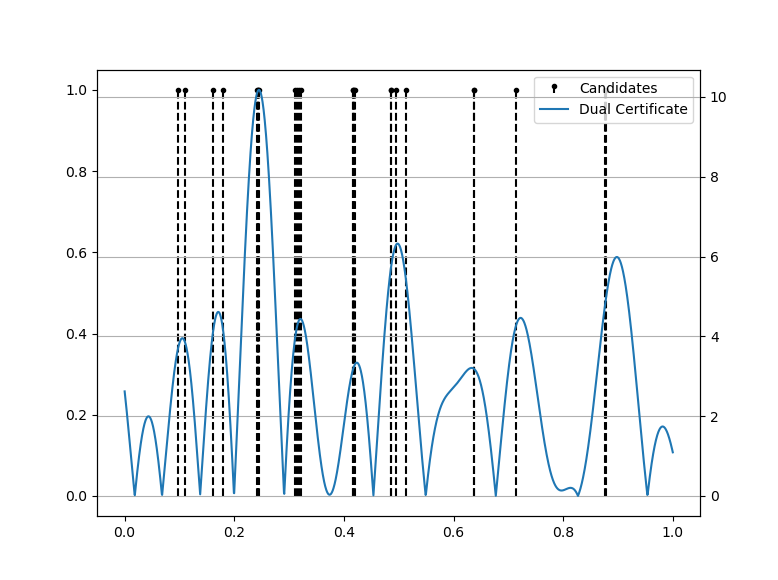
\includegraphics[width=1\linewidth]{swarm.png}
   \caption{Particle swarm optimization candidates with $c1 > c2$}
   \label{fig:swarm} 
\end{subfigure}

\begin{subfigure}[b]{0.8\textwidth}
   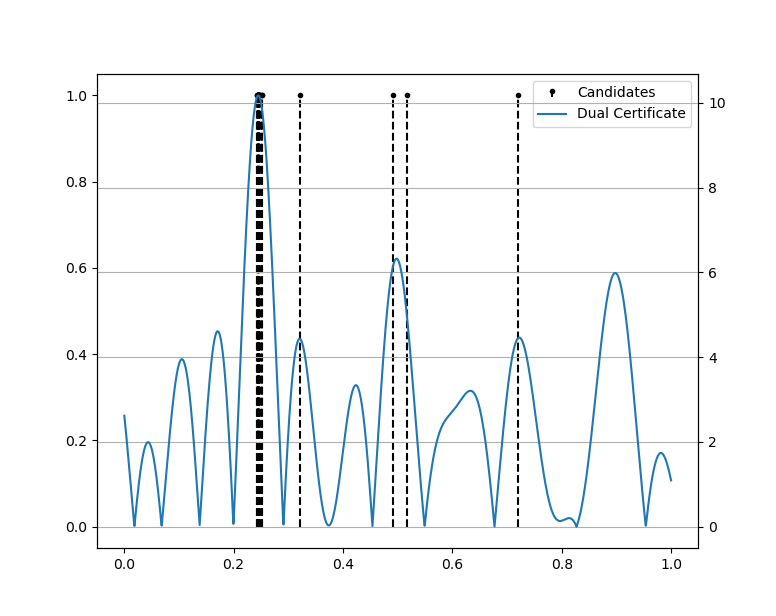
\includegraphics[width=1\linewidth]{swarm2.png}
   \caption{Particle swarm optimization candidates with $c1 < c2$}
   \label{fig:swarm2} 
\end{subfigure}

\caption{Comparing Particle swarm optimization with different coefficient values. Figure \ref{fig:swarm} has a much higher coverage of local maxima and a better spatial diversity than Figure \ref{fig:swarm2}}
\label{fig:swarmvs}
\end{figure}

We can attenuate these limitations by choosing suitable parameters for PSO. There is 2 coefficients parameters $c1$ and $c2$, that manage how much the particles move to the local best ($c1$) or the global best ($c2$). By setting $c1 > c2$, we can have a much higher coverage of local maxima and a better spatial diversity. In Figure \ref{fig:swarmvs}, we show the impact of these coefficients. We still have problems in cases the empirical dual certificate is much harder to optimize (with lots of local maxima) needing a lot of particles and having the PFW do more iterations. Note that in Figure \ref{fig:swarmvs}, the proposed positions are not aligned with the local max, this comes from the difficulty of having a stopping criterion for PSO in our use case. A natural stopping criterion, would be the converge in value of the global max, but this does not mean a converge for other local max. Hence, in practice we run a fixed number of iteration as this algorithm tend to be very fast to converge. This imprecision will slow down the PFW, but it is not a problem as we can refine the candidates in the sub-secant iteration.

\subsection{Particle Gradient Descent}
We introduced the Particle Gradient Descent (p-GD) method, a first-order optimization technique that leverages gradient information to identify local maxima of the empirical dual certificate. In p-GD, a population of particles is initialized across the search space and evolves in parallel, with each particle following the gradient of the empirical dual certificate to converge to the nearest local maximum. With p-GD, we address two shortcomings of PSO, p-GD reliably drives particles toward the nearest local maxima and the method can capture all significant peaks in the empirical dual certificate given a suitable initialization of particles. These local maxima are naturally far enough from each other achieving a sufficient spatial diversity. The main downside of p-GD is that it needs more iterations to converge than PSO making it more costly to compute.

\subsubsection{Initialization}
Initialization plays a critical role in the success of p-GD. Each particle converges to the local maximum within the "valley" it is initialized in. Consequently, for effective candidate selection, particles must be initialized within the valleys corresponding to the desired local maxima. There are 2 trivial initialization methods in p-GD:

\begin{figure}
\centering
\begin{subfigure}[b]{0.9\textwidth}
   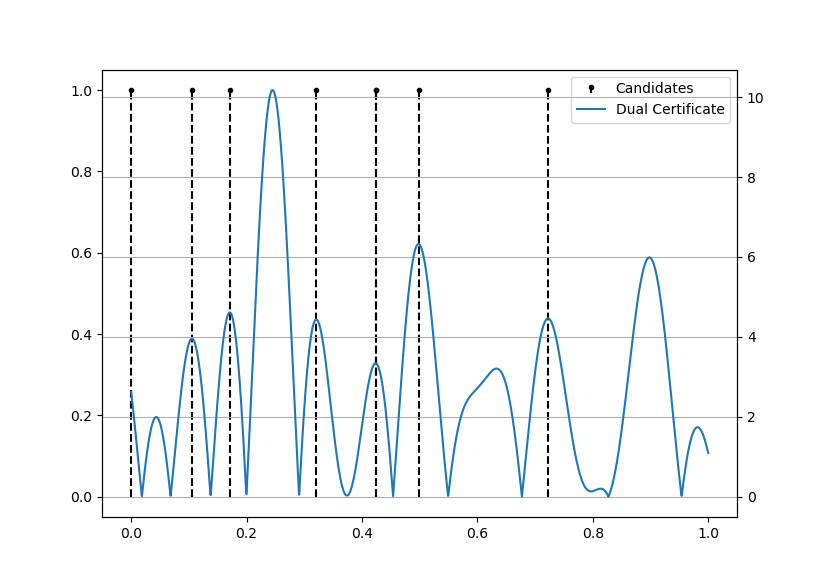
\includegraphics[width=1\linewidth]{random.png}
   \caption{Random initialization}
   \label{fig:random} 
\end{subfigure}

\begin{subfigure}[b]{0.9\textwidth}
   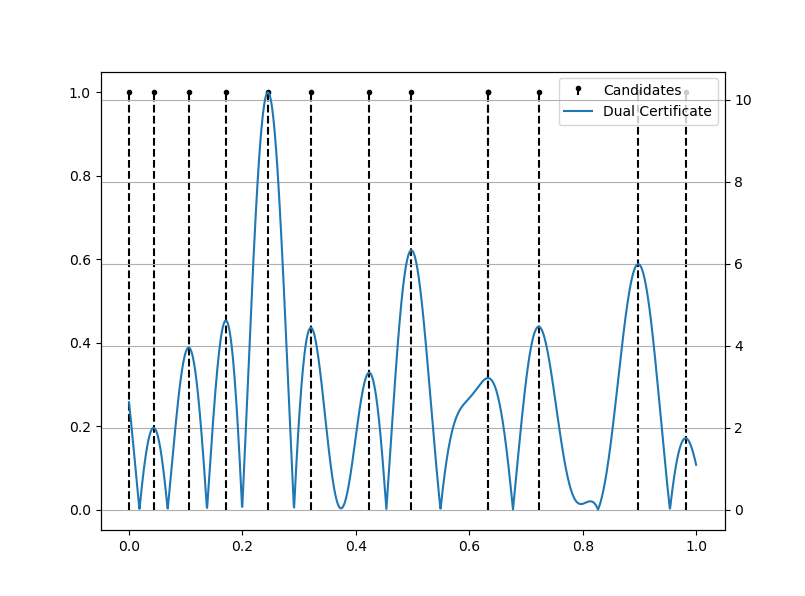
\includegraphics[width=1\linewidth]{grid.png}
   \caption{Grid initialization}
   \label{fig:grid} 
\end{subfigure}

\caption{Comparing Random and Grid initialization.}
\label{fig:randomvsgrid}
\end{figure}

\begin{enumerate}
    \item \textbf{Random}: Particles are distributed randomly within the domain $\mathcal{X}$. This method is faster but lacks guarantees regarding the candidates it identifies, leading to irregular runtime and the possibility of failing to locate the global maximum as shown in Figure \ref{fig:random}. In practice, this leads to the PFW doing more iterations.
    \item  \textbf{Grid}: It initializes particles at a regular intervale inside the domain $\mathcal{X}$ forming a grid. Given that the grid is fine enough, this method finds all local maxima. It is computationally expensive, as a dense grid may result in a large number of particles, making the gradient computation costly and slowing down the correction step. This is particularly problematic for empirical dual certificates with a high number of local maxima, such as those arising from high-frequency Fourier measurements.
\end{enumerate}

A comparison of random and grid initialization methods is shown in Figure \ref{fig:randomvsgrid}. Note that compare to PSO, the grid initialization g-GD gives much better candidates at the cost of a higher computation cost. 

\subsection{Smoothing initialization}
To address the issues with grid initialization, we developed a method named \textit{smoothing initialization}. This approach involves smoothing the empirical dual certificate function by convolving it with a Gaussian kernel, as illustrated in Figure \ref{fig:smoothing_}. The local maxima of this smoothed function are then identified and used as the initial particle positions for the p-GD algorithm, which subsequently refines these points into candidate solutions. \\

This initialization technique drastically reduces the number of candidate points compared to traditional grid initialization, greatly improving the scalability of p-GD in handling high-frequency problems. For instance, as shown in Figures \ref{fig:smoothing} and \ref{fig:smoothing_zoom}, the number of orange crosses (representing initialization points) is much smaller than the total number of local maxima. Importantly, smoothing initialization retains the ability to identify key significant peaks—those that correspond to ground-truth Dirac locations—demonstrated in Figure \ref{fig:smoothing_zoom}. Furthermore, locating the local maxima of the smoothed function is simpler and computationally more efficient.

\begin{figure}
\centering
\begin{subfigure}[b]{0.8\textwidth}
   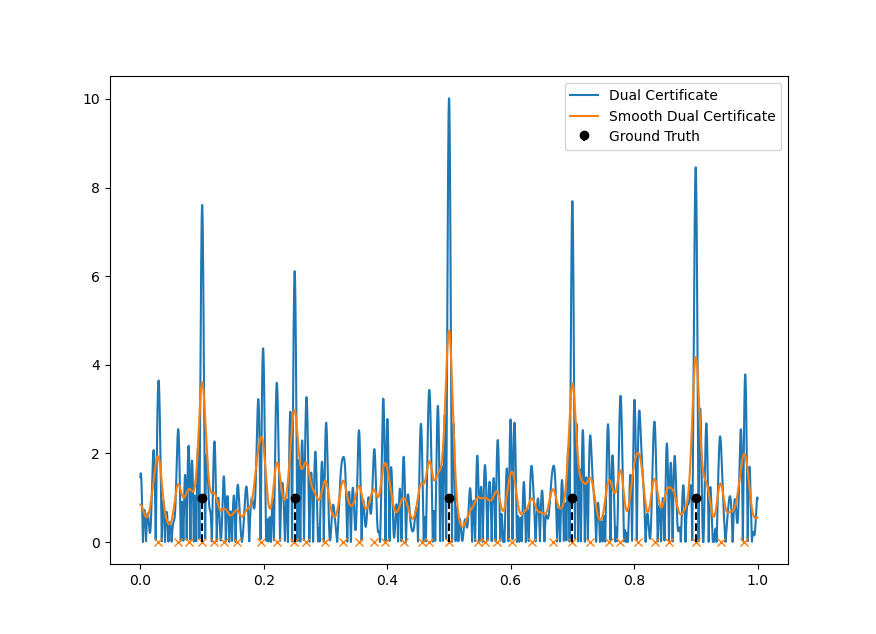
\includegraphics[width=1\linewidth]{smoothing.png}
   \caption{Smoothing of the empirical dual certificate}
   \label{fig:smoothing} 
\end{subfigure}

\begin{subfigure}[b]{0.8\textwidth}
   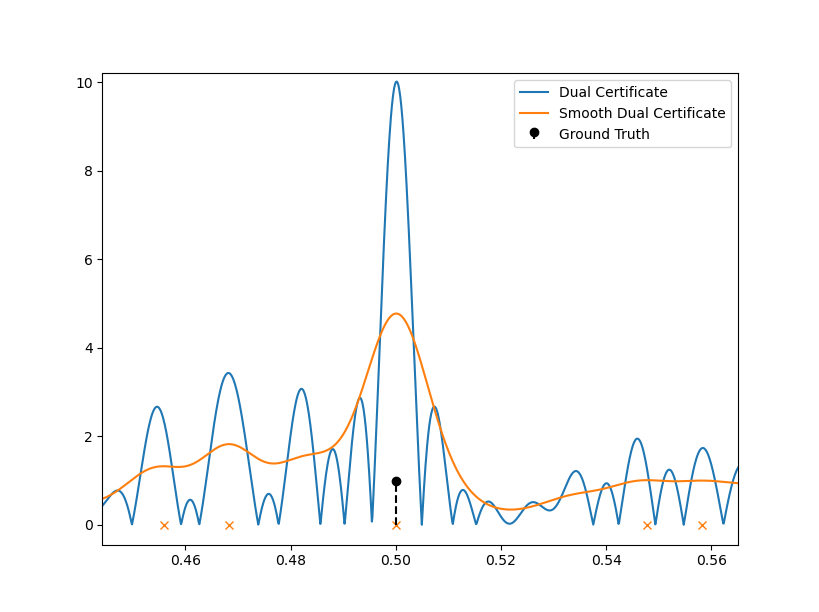
\includegraphics[width=1\linewidth]{smoothing_zoom.png}
   \caption{Zoom of Figure \ref{fig:smoothing}}
   \label{fig:smoothing_zoom} 
\end{subfigure}
\caption{Smoothing of the empirical dual certificate obtain convolution it with a Gaussian kernel from high frequency random Fourier measurements (see Section \ref{operator}). The orange crosses are the initialization points obtain from smoothing on which we run p-GD.}
\label{fig:smoothing_}
\end{figure}

\subsubsection{Numerical methods for smoothing}
We evaluated two numerical approaches for performing the smoothing:

\begin{enumerate}
    \item \textbf{Analytical smoothing}: Deriving an analytical formula for the smoothed empirical dual certificate and then sampling the resulting function on a grid.
    \item \textbf{Discrete smoothing}: Sampling the empirical dual certificate directly on a grid and convolving it with a discrete Gaussian kernel.
\end{enumerate}

In both approaches, the outcome is a discrete, smoothed empirical dual certificate represented on a grid, which scales with the frequency of the operator (i.e. how much the empirical dual certificate varies). The initialization points (orange crosses) are then determined using existing numerical peak-finding methods. Both methods have comparable computational costs. However, after thorough testing, we found that Discrete Smoothing yielded better results, producing fewer initialization points.

\section{Ilustration of the polyatomic Frank-Wolfe mechanisms}
To conclude this section on the description of the polyatomic Frank-Wolfe algorithm, we propose here to illustrate the mechanisms at play by observing the successive iterates during one reconstruction. We use one of the experimental setups presented further down in details in section \ref{setup}. The main objective for now is to illustrate the candidate selection and correction step, which is valid for all experimental setups and candidate selection methods considered. \\

In Figure \ref{fig:reconstruction}, we plotted the reconstruction iteration wise. The first column correspond the Candidate Search step of PFW and show the empirical dual certificate we use to find the candidates. We plot the smoothed dual certificate and the candidates $\mathbf{x}^{[k]}_{candidates}$ that are proposed to the correction step. The second column shows the reconstruction signal $\mathbf{x}^{[k]}, \mathbf{a}^{[k]}$ after the correction step. \\

Iteration 1 highlights how the correction step filters the candidates, as discussed in Section \ref{correction}. Iteration 2 demonstrates the thresholding mechanism which eliminates candidates value $|\eta^{[k]}| < 1$ before passing them to the correction step. Looking at the reconstruction $\mathbf{x}^{[k]}, \mathbf{a}^{[k]}$ at each iteration, we note how the PFW keeps adding new spikes and removing old ones via the correction step, maintaining an improved solution, thus having the empirical dual certificate converge to 1 at the Dirac's positions. It is important to note that, in most cases, the algorithm reconstructs a spike with multiples ones. This occurs because the sliding step from SFW is absent.

In Figure \ref{fig:reconstruction2}, we do the same reconstruction using a positivity
constraint. It show how well behave the empirical dual certificate is without the absolute value and how easier the Candidate Search becomes, while giving the same solution.

\begin{figure}[t!]
\centering
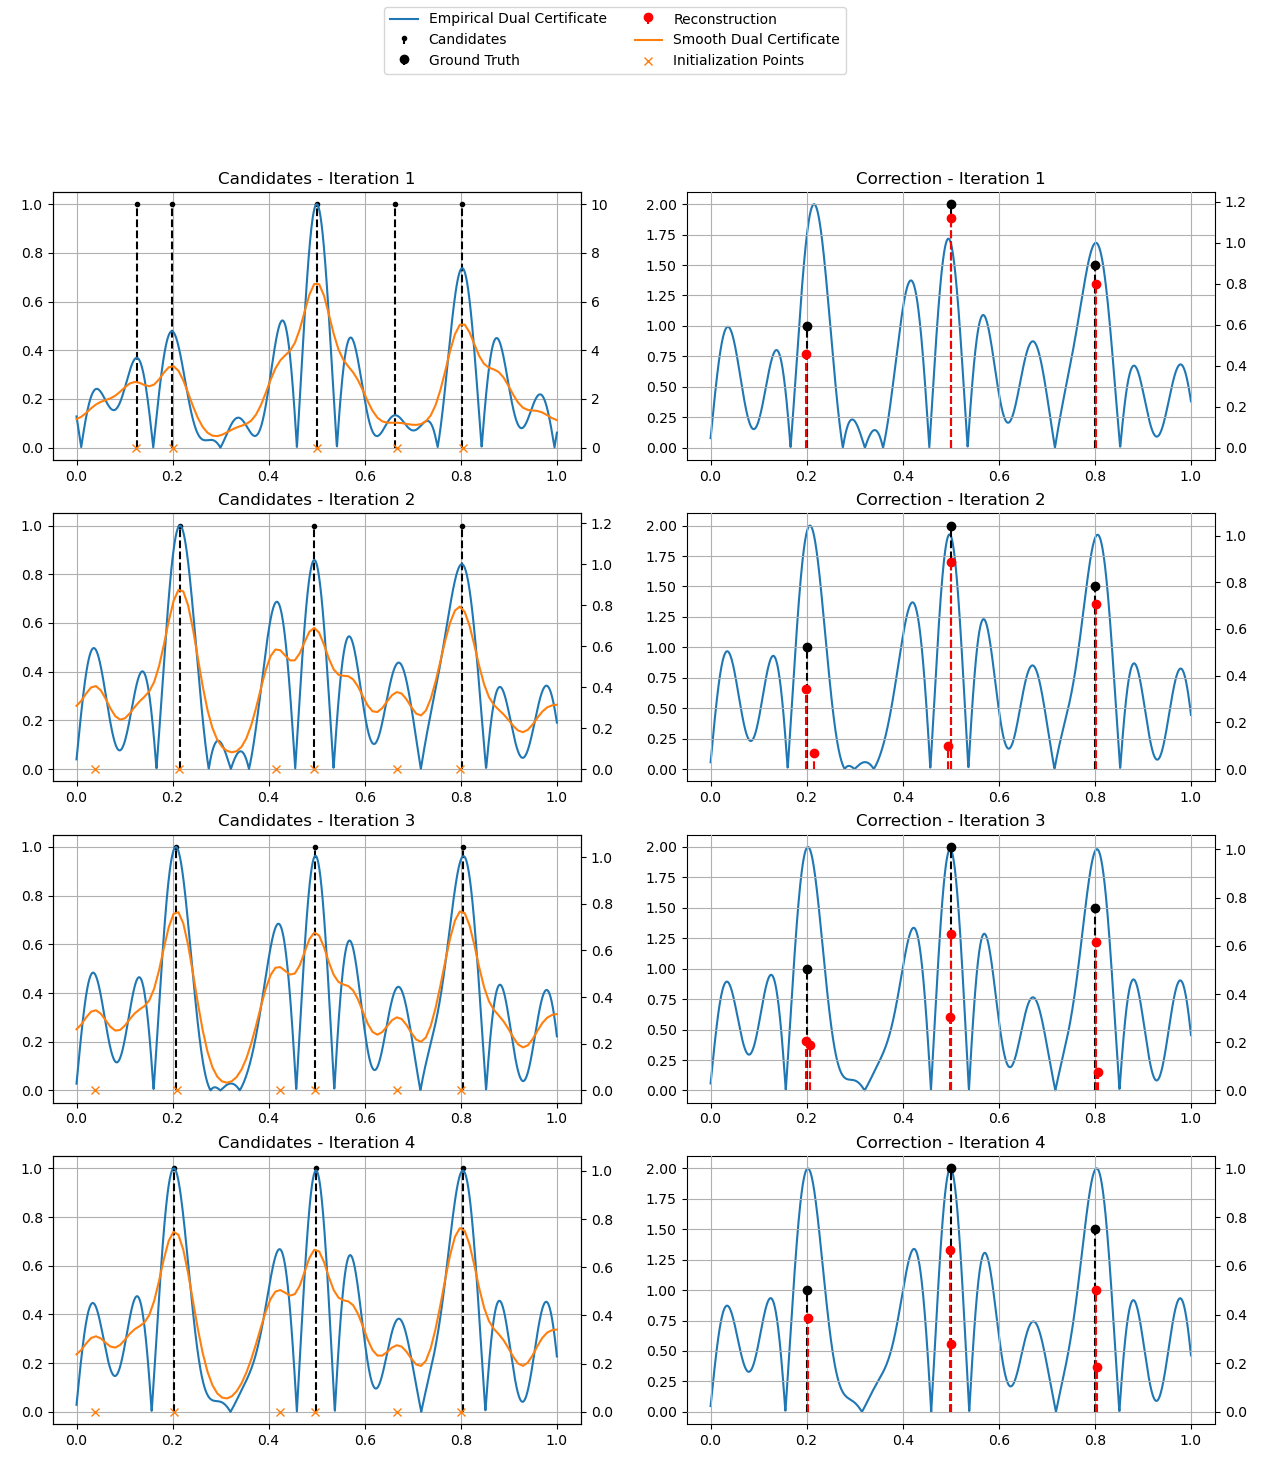
\includegraphics[width=1\linewidth]{reconstruction.png}
\caption{Reconstruction iteration by iteration using polyatomic Frank-Wolfe algorithm (with smoothing). The first column correspond the Candidate Search step and the second show the reconstruction after the correction step. For all plots, the left y axis correspond to the value of the Diracs and the right y axis correspond to the empirical dual certificate.}
\label{fig:reconstruction}
\end{figure}

\begin{figure}[t!]
\centering
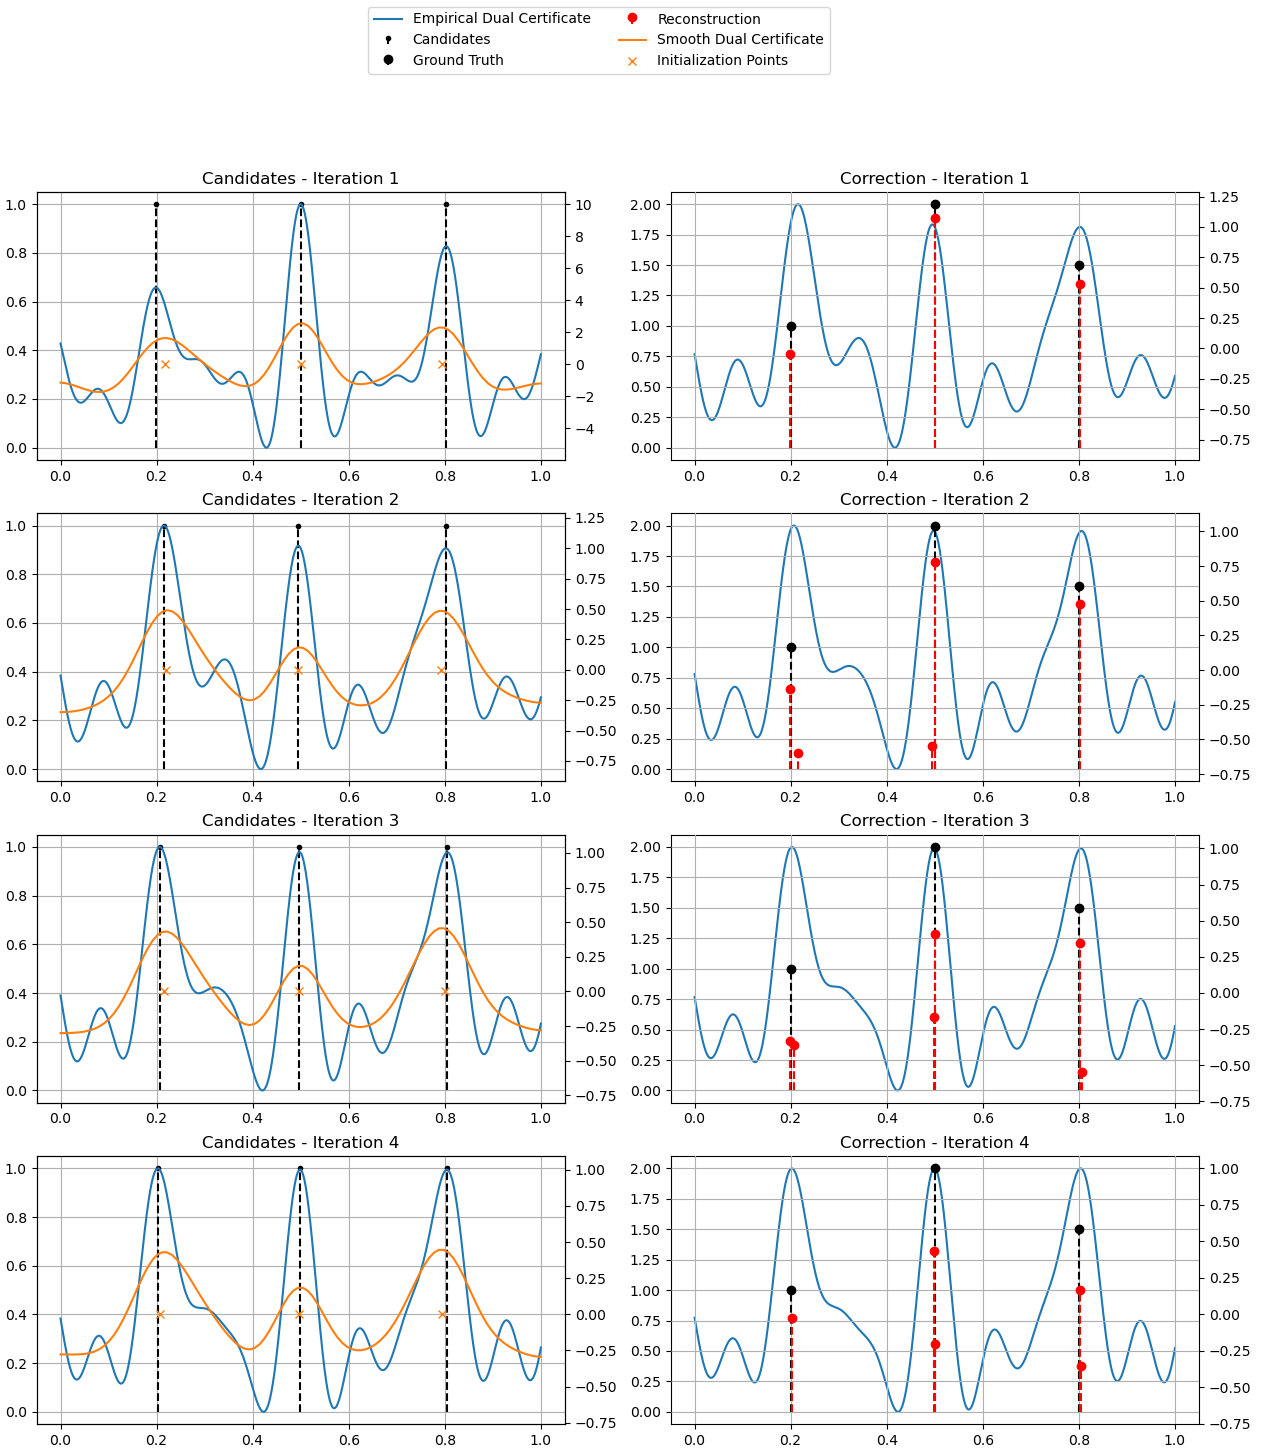
\includegraphics[width=1\linewidth]{reconstruction2.png}
\caption{Same reconstruction has Figure \ref{fig:reconstruction}, but using a positivity constraint.}
\label{fig:reconstruction2}
\end{figure}

\chapter{Numerical experiments and Results}
In this chapter, we evaluate the performance of the the polyatomic Frank-Wolfe algorithm through multiple experiments. These experiments demonstrate the numerical effectiveness of the algorithm and provide insights into its advantages and limitations. We analyze the performance of various candidate selection methods and provide a comparison between the PFW and the SFW baseline algorithm. 

\section{Setup} \label{setup}
Before delving into the results, we outline the experimental setup, including the forward operator, the noise level, the regularization parameter $\lambda$ and the ground truth signal.

\subsection{Forward operator} \label{operator}
We consider 2 different operator, the random Fourier operator and a convolution operator. For each operator we define its forward $\Phi_\mathbf{x}$ and its adjoint $\Phi^*$. We always define the operator $\Phi_\mathbf{x}$ with a vector $x$ which are the positions of the Diracs. As $\Phi m$ is not linear in $m$, making math simpler. Also, in the PFW algorithm we only need $\Phi_\mathbf{x}$. The adjoint $\Phi^*$ is a function since $\mathcal{M}(\mathcal{X})$ can be seen as the topological dual of $\mathcal{C}_0(\mathcal{X})$ (see Section \ref{ssr}).\\

The operators are defined by equation $\Phi m \stackrel{def}{=} \int_{\mathcal{X}} \varphi(x) dm(x)$ \eqref{measurements} with the corresponding kernel $\varphi$ and by setting $m = \sum_{i = 0}^{N} a_i \delta_{x_i}.$

\subsubsection{Random Fourier operator}
We define the Fourier operator for a random frequency $w_i$ with $|w_i| \leq f_{max}$. The vector $\mathbf{w} \in \mathbb{R}^M$ contains all the measured random frequency. \\

We use the Fourier kernel $\varphi(x) = e^{-2j \pi x w_i}$ and obtain:

\begin{equation}
\begin{split}
    \Phi_\mathbf{x} (\mathbf{a})(w_i) &= \sum_{k = 1}^{n} a_k e^{-2j \pi x_k w_i} \\
    \Phi^*(\mathbf{y})(t) &= \sum_{k = 1}^{n} y_k e^{2j \pi t w_k}
\end{split}
\end{equation}

\subsubsection{Convolution operator}
We define the Convolution operator for a position $z_i \in \mathcal{X}$. The vector $\mathbf{z} \in \mathcal{X}^M$ is a sampling grid and we sample the convolution of the signal with a Gaussian. \\

We use the convolution kernel $\varphi(x) = \frac{1}{\sqrt{2 \pi} \sigma} e^{\frac{-(z_i - x)^2}{2\sigma^2}}$ and obtain:
\begin{equation}
\begin{split}
    \Phi_\mathbf{x} (\mathbf{a})(z_i) &= \sum_{k = 1}^{n} a_k \frac{1}{\sqrt{2 \pi} \sigma} e^{\frac{-(z_i - x_k)^2}{2\sigma^2}} \\
    \Phi^* (\mathbf{y})(t) &= \sum_{k = 1}^{n} y_k \frac{1}{\sqrt{2 \pi} \sigma} e^{\frac{-(z_k - t)^2}{2\sigma^2}}
\end{split}
\end{equation}

In both case, $\mathbf{a} \in \mathbb{R}^N$ is the vector of amplitudes, $\mathbf{y} \in \mathbb{R}^M$ the measurements vector, $t \in \mathcal{X}$ the variable of the function $\Phi^* (\mathbf{y})$.\\

The number of measurements $M$ is important and different for both operators. For Fourier, we take a number of measurements proportional to the number of spikes in the ground truth, $M = 10 N$ with $N$ the number of spikes. For convolution, we have to a parameter, the full width at half maximum (FWHM), we can link the standard deviation $\sigma$ with the FWHM by $FWHM = 2 \sqrt{2\ln2} \sigma$. To have realistic measurements we need a distance between the grid points also called pixel size of $\leq FWHM / 3$. Meaning that $M \propto 3 / FWHM$. The value 3 is a minium value, we can have a better definition with a number $\geq 3$.

\subsection{Noise and regularization}
To have more realistic results we need to add noise to our experiments and have a sutable regularization parameter $\lambda$. We choose to add an additive Gaussian white noise with a PSNR of 20 dB for all experiments. For the regularization, we choose a method to auto-scale $\lambda$ with respect to the problem size. There exists a critical value $\lambda_{max}$ such that, for any larger values $\lambda \geq \lambda_{max}$, the solution to the BLASSO is $m=0$ (see \cite{9258416} Proposition II.1). So we choose the value of $\lambda$ as a fraction of $\lambda_{max}$: 

\begin{equation}
    \lambda = \alpha \lambda_{max}= \alpha ||\Phi^*\mathbf{y}||_\infty
\end{equation}

with $ 0 \leq \alpha \leq 1$ a factor that depends on the noise level. The typical value of $\alpha$ belongs to the range $[0.01, 0.15]$.
For our experiments, we choose to take $\alpha = 0.1$.

\begin{figure}
\centering
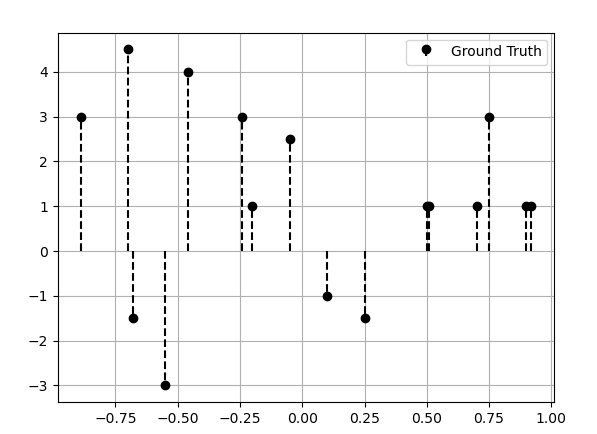
\includegraphics[width=1\linewidth]{GT.png}
\caption{Ground truth signal for 1D experiments. It contains 16 peaks with amplitude from -5 to 5.}
\label{fig:GT}
\end{figure}

\subsection{Signal to reconstruct}
In all 1D experiments, we reconstruct the signal shown in Figure \ref{fig:GT}. For 2D deconvolution, we use the signal shown later in Figure \ref{fig:gt_2d} and use only positive amplitudes. 

\section{1D Fourier reconstruction}
In this section, we showcase the polyatomic Frank-Wolfe algorithm performance, behavior and providing insights into its advantages and limitations in the case of 1D reconstruction using random Fourier measurements. In the experiments, we consider 3 different $f_{max}$ to demonstrate the algorithm in different situations. We define low, high and very high frequency settings such that $f_{max}^{very\_high} = 10 f_{max}^{high} = 100 f_{max}^{low}$. We show in Figure \ref{fig:smoothing_reconstruction}, how the $f_{max}$ can impact the reconstruction. In particular, higher frequency measurement has a much more accurate reconstruction. 

\begin{figure}
\centering
\begin{subfigure}[b]{1\textwidth}
   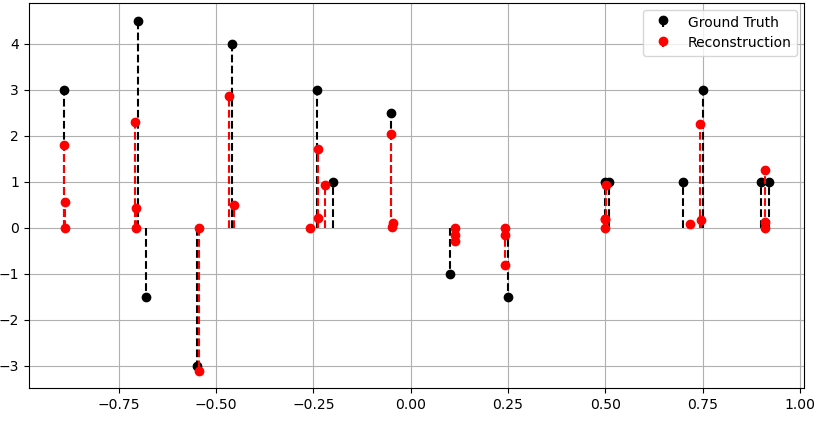
\includegraphics[width=1\linewidth]{smoothing_low.png}
   \caption{Reconstruction of Low Frequency}
   \label{fig:smoothing_low} 
\end{subfigure}

\begin{subfigure}[b]{1\textwidth}
   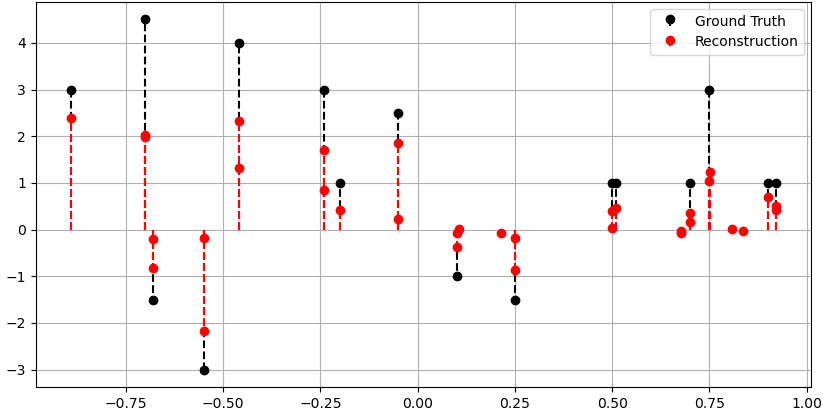
\includegraphics[width=1\linewidth]{smoothing_high.png}
   \caption{Reconstruction of High Frequency}
   \label{fig:smoothing_high} 
\end{subfigure}

\caption{Reconstruction of the signal shown in Figure \ref{fig:GT} using a 1D Random Fourier operator and using p-GD with smoothing initialization.}
\label{fig:smoothing_reconstruction}
\end{figure}

\subsection{Reconstruction: SFW vs PFW}

In Figure \ref{fig:PFWvsSFW}, we compare the reconstruction of the PFW and the SFW. In both cases the reconstruct is very accurate and similar. The only difference is that PFW tends to reconstruct each Dirac with multiple spikes while SFW only reconstructs one, having a sparser solution. The sliding step form the sliding Frank-Wolfe algorithm is necessary to have spare solutions, it was already suggested in \cite{Bredies2012}, and strongly advocated in \cite{Boyd2015}, to modify the Frank-Wolfe algorithm and to let the Dirac positions move.\\

Without this step, our PFW generates solution that are not very sparse, but it can be solved by doing some post processing  treatment to merge those spikes. Specifically, by merge those spikes into a center of mass Dirac in between, one can "recover" the SFW solution as shown in Figure \ref{fig:PFWvsSFW_cm}. In practice, we see a convergence to the solution of the SFW. This post processing step is very cheap and much cheaper than doing a sliding step and is one of the advantages of doing polyatomic updates. Indeed, with polyatomic updates we can add a lots of Diracs to the solution at each iteration. While if we restrict ourself to atomic updates similar to SFW without a sliding step then the algorithm would need much more iterations thus the need of this additional step. We also tried to replace the sliding step by a merging step at each iteration without success. We did not research other methods to solve this problem as this post processing was sufficient for us, but it remains an area of improvements for PFW.


\begin{figure}
\centering
\begin{subfigure}[b]{1\textwidth}
   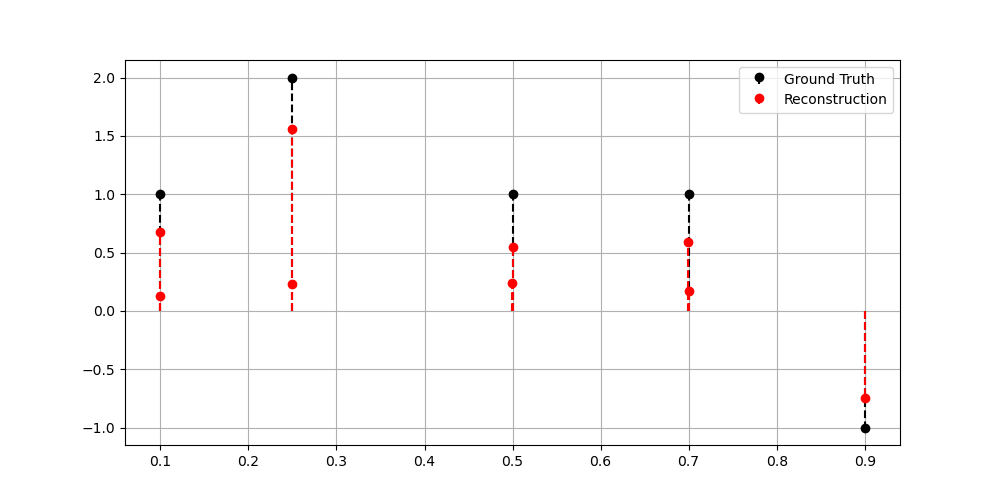
\includegraphics[width=1\linewidth]{PFW.png}
   \caption{Polyatomic Frank-Wolfe solution}
   \label{fig:PFW} 
\end{subfigure}

\begin{subfigure}[b]{1\textwidth}
   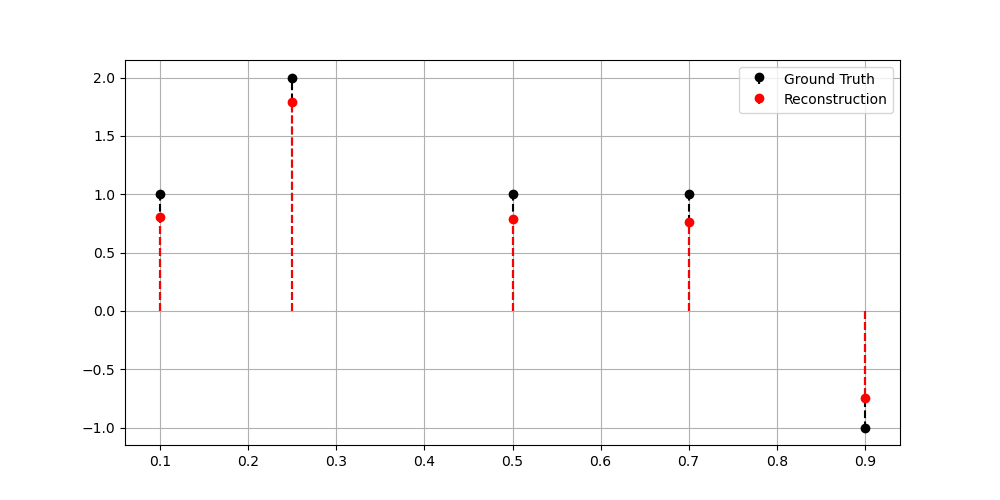
\includegraphics[width=1\linewidth]{SFW.png}
   \caption{Sliding Frank-Wolfe solution}
   \label{fig:SFW}
\end{subfigure}

\caption{Reconstruction by PFW and SFW for a 1D random Fourier operator with noise. Both have very similar and accurate reconstruction. Without the sliding step from SFW, PFW reconstructs each spikes with multiple Diracs.}
\label{fig:PFWvsSFW}
\end{figure}

\begin{figure}
\centering
\begin{subfigure}[b]{1\textwidth}
   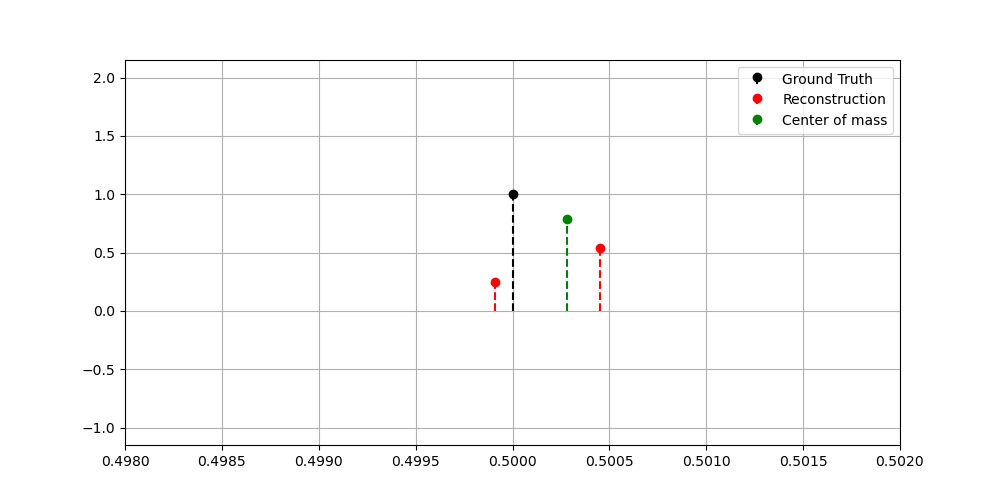
\includegraphics[width=1\linewidth]{PFW_cm.png}
   \caption{Zoom of the PFW solution in Figure \ref{fig:PFW}}
   \label{fig:PFW_cm} 
\end{subfigure}

\begin{subfigure}[b]{1\textwidth}
   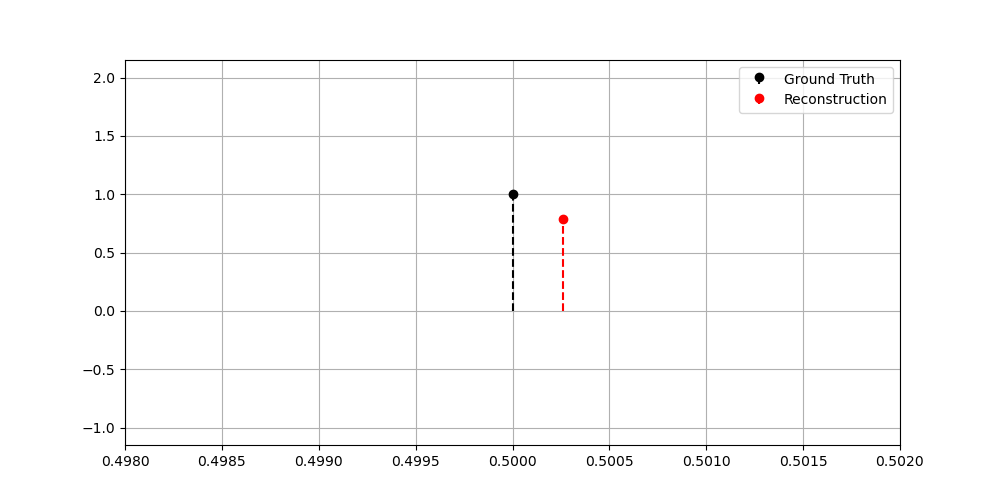
\includegraphics[width=1\linewidth]{SFW_cm.png}
   \caption{Zoom of the SFW solution in Figure \ref{fig:SFW}}
   \label{fig:SFW_cm}
\end{subfigure}

\caption{Zooming in to the reconstruction of Figure \ref{fig:PFWvsSFW}. The center of mass of the PFW solution is almost the same as the SFW.}
\label{fig:PFWvsSFW_cm}
\end{figure}

\subsection{Compare Candidates Search Methods}
The first numerical experiment is to compare the different candidates selection methods. There is 4 methods, PSO and p-GD with the 3 different (random, grid and smoothing) initialization. We show the time in seconds the algorithms takes to run in Table \ref{table:cs} and the same results split into the 2-steps of the PFW algorithm are shown in Table \ref{table:cs2}. \\

\begin{table}
  \centering
  \renewcommand{\arraystretch}{1.2}
  \begin{tabular}{|p{2cm}|ccc|}
    \hline
    \multirow{2}{3cm}{\textbf{Time (s)}} & \multirow{2}{2.5cm}{\textbf{Low Frequency}} & \multirow{2}{3cm}{\textbf{High Frequency}} & \multirow{2}{3cm}{\textbf{Very High Frequency}}\\
     &  &  &   \\
    \hline
    PSO & 4.18 & 8.59 & 11.58   \\ \hline
    Random & 1.10 & 4.37 & 17.97\\ \hline
    Grid & 1.50 & 5.32 & 40.82  \\ \hline
    Smoothing  & \textbf{0.93} & \textbf{2.80} & \textbf{4.53} \\ \hline
  \end{tabular}
  \caption{Time in seconds the PFW takes to run for the four Candidates Search methods presented. We show the results for 3 different $f_{max}$.}
  \label{table:cs}
\end{table}

\begin{table}
  \centering
  \renewcommand{\arraystretch}{1.2}
  \begin{tabular}{|p{2cm}|ccc|ccc|}
    \hline
    \multirow{2}{3cm}{\textbf{Time (s)}} & \multicolumn{3}{c|}{\textbf{Candidates Search}} & \multicolumn{3}{c|}{\textbf{Correction}}\\

    \cline{2-7}
    & \textbf{Low} & \textbf{High} & \textbf{Very High} & \textbf{Low} & \textbf{High} & \textbf{Very High} \\
    \hline
    PSO & \textbf{0.07} & \textbf{0.28} & \textbf{1.63} & 3.90 & 7.96 & 9.72 \\ \hline
    Random & 0.40 & 1.91 & 14.51 & 0.51  & 2.32 & 3.26 \\ \hline
    Grid & 0.63 & 3.27 & 36.66 & 0.78 & 1.96 & 4.06 \\ \hline
    Smoothing & 0.29 & 0.72 & 1.71 & \textbf{0.52} & \textbf{1.97} &  \textbf{2.76} \\ \hline
  \end{tabular}
  \caption{Same results as Table \ref{table:cs}, split into the 2 steps of the PFW algorithm.}
  \label{table:cs2}
\end{table}


The p-GD with smoothing initialization is better then all other methods in all cases. Especially for very high frequency measurements where it largely beats others and has the best scaling. It is an expected results as smoothing was design for dual certificate that are high frequency. It also is very fast comparable to PSO, because the smoothing finds a low number of candidates.  Looking at Table \ref{table:cs2}, PSO can still beats all p-GD methods for candidates search, but it overall slower because the correction is badly conditioned, as said beofre the candidates lacks spatial diversity. Both PSO and random are faster than grid method, even if they take more iteration of the algorithm to run, but both lack local maxima coverage leading to irregular runtime. Grid is the slowest because it need a grid that is fine enough leading to a high number of candidates that make running the gradient descent very expensive. Overall the take away here is that smoothing is a good idea to find candidates. While  p-GD with smoothing is good enough for us, there is still a big research area here to find even better candidates. It can be using the dual certificate or even using another mathematical approaches.

\subsection{Baseline comparison}
The second numerical experiment compares the PFW algorithm against a baseline. For this purpose, we select the SFW algorithm as the baseline, as it represents a state-of-the-art approach for solving BLASSO and serves as the foundational algorithm upon which PFW is designed. We do the same experiment as above with 3 different $f_{max}$. We choose 4 algorithm to test namely SFW using p-GD with smoothing initialization to find the global maximum, SFW using PSO, PFW also using p-GD with smoothing initialization and lastly a mix between PFW and SFW which is the PFW algorithm with a sliding step. The time in seconds the 4 algorithms takes to run are shown in Table \ref{table:PFWvsSFW} and the same results split into the 3-steps (Candidates
Search, Correction and Sliding) are shown in Table \ref{table:PFWvsSFW2}.\\

\begin{table}
  \centering
  \renewcommand{\arraystretch}{1.2}
  \begin{tabular}{|p{2.5cm}|ccc|}
    \hline
    \multirow{2}{3cm}{\textbf{Time (s)}} & \multirow{2}{2.5cm}{\textbf{Low Frequency}} & \multirow{2}{3cm}{\textbf{High Frequency}} & \multirow{2}{3cm}{\textbf{Very High Frequency}}\\
     &  &  &   \\
    \hline
    Sliding FW & 1.82 & 5.19 & 15.79   \\ \hline
    Sliding FW + PSO & 1.45 & 2.46 & 6.44   \\ \hline
    Polyatomic FW & 0.93 & 2.8 & 4.53 \\ \hline
    PFW + Sliding & \textbf{0.67} & \textbf{2.32} & \textbf{4.38}\\ \hline
  \end{tabular}
  \caption{Time in seconds to run for the four algorithms benchmarked. We show the results for 3 different $f_{max}$.}
  \label{table:PFWvsSFW}
\end{table}

\begin{table}
\centering
\renewcommand{\arraystretch}{1.1}
\begin{tabular}{|p{2.75cm}|l|c|c|c|c|}
\hline
\multirow{2}{2cm}{Time (s)} & \multirow{2}{2cm}{Frequency} & \multirow{2}{2cm}{Candidates Search} & \multirow{2}{2cm}{Correction} &  \multirow{2}{1.25cm}{Sliding} &  \multirow{2}{2cm}{Number of Iterations}\\
 &  &  &  &  &  \\
\hline
\multirow[t]{3}{*}{Sliding FW} 
& Low & 0.70 & 0.24 & 0.57 &  13 \\
 & High & 2.61 & 0.55 & 1.59 &  21 \\
 & Very High & 13.09 & \textbf{0.50} & 1.74 & 20 \\
\cline{1-6}
\multirow[t]{3}{*}{SFW + PSO}
& Low & \textbf{0.10} & 0.30 & 0.76 & 14 \\
& High & \textbf{0.31} & \textbf{0.37} & 1.33 & 20 \\
& Very High & 2.91 & 0.58 & 2.42 & 23 \\
\cline{1-6}
\multirow[t]{3}{*}{Polyatomic FW}
& Low & 0.29 & 0.52 & - & \textbf{4} \\
& High & 0.72 & 1.97 & - & 4 \\
& Very High & \textbf{1.71} & 2.76 & - & \textbf{3} \\
\cline{1-6}
\multirow[t]{3}{*}{PFW + Sliding}
& Low & 0.16 & \textbf{0.11} & \textbf{0.35} & \textbf{4}\\
& High & 0.47 & 1.23 &  \textbf{0.56} & \textbf{3}\\
& Very High & 1.81 & 1.39 &  \textbf{1.10} & \textbf{3}\\
\hline
\end{tabular}
  \caption{Same results as Table \ref{table:cs}, split into the 3-steps (Candidates Search, Correction and Sliding) and with the number of iteration the algorithm has done.}
  \label{table:PFWvsSFW2}
\end{table}

The results are a bit more mitigated than before, we can still see that doing polyatomic updates is better than a single atom update, up to 4x faster. With the same candidate selection method PFW is much better than SFW, but SFW can beat PFW as it may have a faster method to find the global maximum of the empirical dual certificate. The main advantage of PFW is the convergence speed, the algorithm needs much less iterations to converge to the solution. PFW really shines when the signal has numerous Dircas to reconstruct as SFW will run a number of iteration equals to the number of spikes. Table \ref{table:PFWvsSFW}, also shows that PFW + sliding is better than PFW, but it mainly depends on how much the sliding step cost. Remember that the sliding step is increasingly costly with a lot of spikes or in high dimensions.\\

Looking at Table \ref{table:PFWvsSFW2}, we can see the bottleneck of the different algorithm. For SFW, the main bottleneck are the high number of iteration compare to PFW. It means that even if the candidate search step and the sliding step are computational cheaper, overall it costs more to run than the PFW. For PFW, both step of the algorithm are expensive. In practice, the correction step computation is highly variable often need 10 to 100 times more FISTA's iterations compared to SFW. It is mainly due to the fact that we propose multiples update direction and thus need more work to find their weights. The candidates search step is also expensive because of the high number of particle that run the gradient descent.

\subsection{Spikes scaling} \label{spikes_scaling}
In this section, we want to study in more details in which regime the PFW shines. As discussed above, PFW converges much faster compare to the $N$-step converge of the SFW and thus the regime at which PFW shines is when we have a lot of spikes to reconstruct. So we made an experiment where the number of Diracs varies. Specifically, we create random signals with a varying number spikes and use the four algorithms mentions above to reconstruct this signal from 1D random Fourier measurements. In Table \ref{fig:n_spikes}, we shown the time in seconds each algorithm takes to run (y ax) for different number of spikes (x ax). \\

\begin{figure}[]
\centering
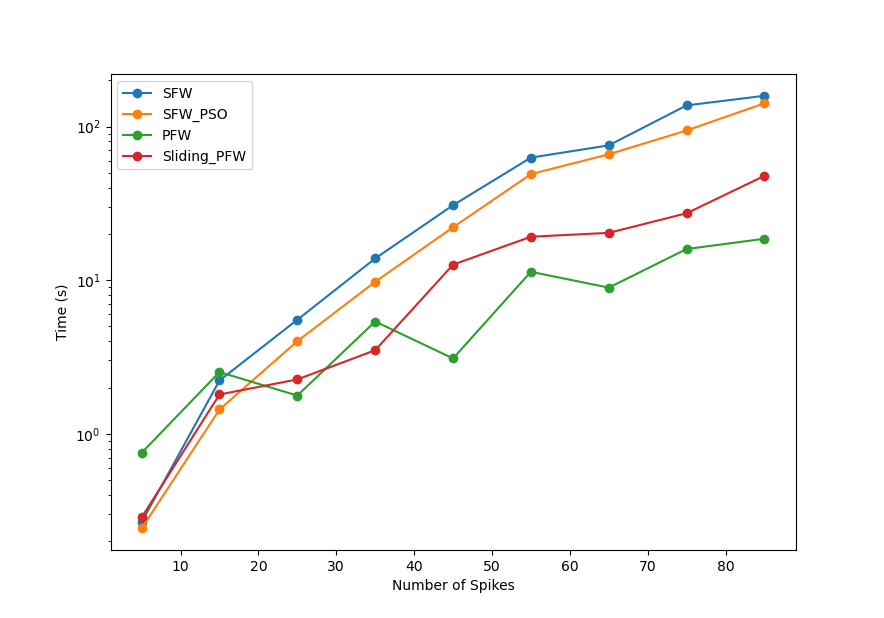
\includegraphics[width=1\linewidth]{n_spikes.png}
\caption{Time in seconds to run for the four algorithms benchmarked with a varying number Diracs to reconstruct.}
\label{fig:n_spikes}
\end{figure}

Globally the compute increases with the number of spikes increase, due to increasing problem size, the Fourier operator takes more measurements with more spikes. At $15$ spikes we have a critical point where for signals with $<15$ spikes, SFW is more efficient while for $>15$ spikes signals, PFW is better. Starting from around 50 spikes we have a 10x difference between both. The PFW variant with sliding can keep up with PFW mainly due to having polyatomic update direction, while its scaling is worse than PFW because of the expensive sliding step. \\

In Table \ref{fig:n_spikes2}, we show the same results split between the $3$-steps (Candidates Search, Correction and Sliding) for PFW and SFW. It shows the bottleneck of both algorithms. For PFW, the correction step is dominant over the candidate search step and has a highly variable computation due the to the condition of $\Phi_x$. For SFW, the correction step computation is almost negligible, the candidate search step and the sliding step are both the bottleneck. It shows the bad scaling of the sliding step, it is the cheapest for 5 spikes and the most expensive for 95 spikes, 20x more spikes leads to 1000x more computation time. This exponential scaling is one of the reason to remove the sliding from PFW. For both algorithms, the computation of the candidate search step is heavy influenced by the frequency of the Fourier operator and not much influenced by the number of spikes.

\begin{figure}
\centering
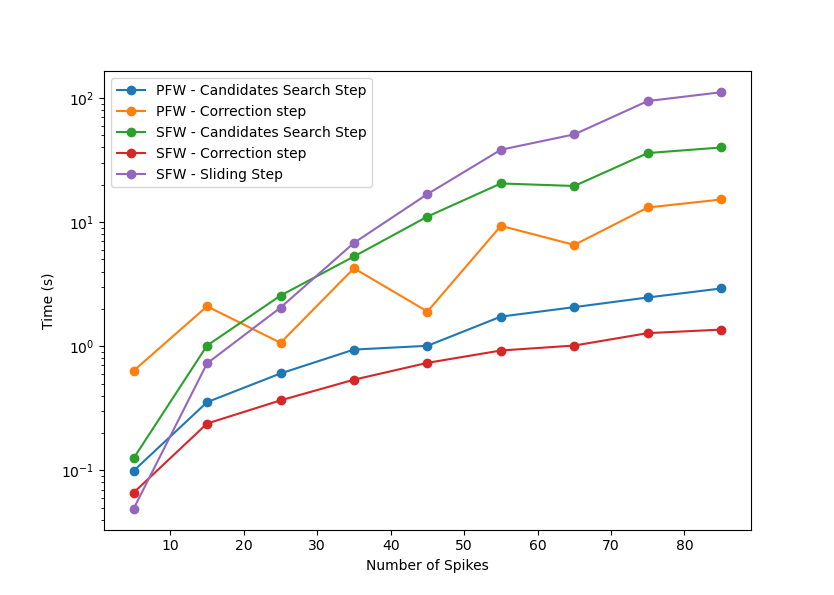
\includegraphics[width=1\linewidth]{n_spikes2.png}
\caption{Same results as Table \ref{fig:n_spikes}, split into the 3-steps (Candidates Search, Correction and Sliding) for PFW and SFW.}
\label{fig:n_spikes2}
\end{figure}

\subsection{Metric Baseline comparison}
We have shown the computational performance of the algorithm, now we want to showcase the accuracy of the algorithm in finding the solution. To do so, we use a metric to assess the performance of reconstruction and compare PFW with SFW.

\paragraph{Flat norm}
\begin{figure}
\centering
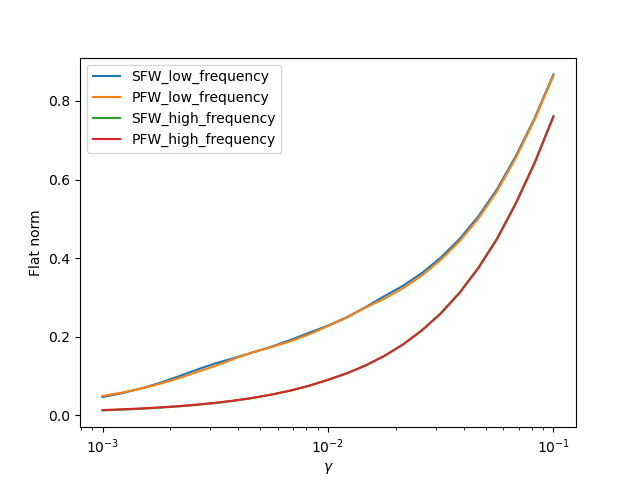
\includegraphics[width=0.9\linewidth]{falt_norm.png}
\caption{Flat norm value (lower better) for different value of $\gamma$ comparing the reconstruction of both PFW and SFW using low and high frequency Fourier measurements.}
\label{fig:flat_norm}
\end{figure}

The metric we use is the so-called \textit{flat norm} introduced in \cite{denoyelle2021optimaltransportbasedmetricsmlm}. The flat norm or also called flat metric is an optimal transport-based metric for measures that depends on a parameter $\gamma$. It can be seen as an interpolating distance between the 1-Wasserstein distance $||\cdot||_{W_1}$ \cite{ramdas2015wassersteinsampletestingrelated} and the total variation norm $||\cdot||_{\mathcal{M}}$, with interpolating parameter $\gamma$. When $\gamma \xrightarrow{} + \infty$ we recover the 1-Wasserstein distance and when $\gamma \xrightarrow{} 0$ we recover the total-variation norm. For a reconstructed Dirac, we can interpret this metric as the cost of transporting the Dirac mass to the ground truth if the distance between both spikes is $< \gamma$ and if the distance is $> \gamma$, the metric accounts for the destruction and creation of mass such that the reconstructed Dirac is destroyed and recreated at the right location. \\


We use the flat norm to compare the reconstruction of both PFW and SFW in the cases of low and high frequency Fourier measurements. Figure \ref{fig:flat_norm} shows the flat norm value for different value of $\gamma$. Both PFW and SFW have almost the same reconstruction quality and there is no visible difference in term of flat norm. Only by taking higher frequency measurements can we increase the quantity of the reconstruction. 

\section{2D Deconvolution}
In this section, we showcase the polyatomic Frank-Wolfe algorithm in another settings, 2D deconvolution. Reconstrution in 2D means that the Diracs now lives in a 2D space and have 2 coordinates to recover. This 2D space heavy influence the algorithm efficiency as the search candidates space is now squared. For examples, both grid and smoothing initialization have a squared grid compare to 1D case. The convolution operator also behaves very differently from the Fourier one. The Fourier operator has a number of measurements that is proportional to the number of spikes in the signal and the quality of the reconstruction influenced by the maximum frequency. For the convolution operator, both the number of measurements and quality depends on FWHM (i.e. width of the Gaussian kernel) and the definition (i.e. the pixel size or number of measurements per Gaussian).

\subsection{Simulated single molecule localization microscopy}

We tried to simulate the practical settings of super-resolution for microscopy. In super-resolution, one wants to retrieve some fine scale details to better study biological structures of interest. The studied bodies are generally smaller than the Rayleigh limit at 200 nm, a length at which the phenomenon of light diffraction comes into play. This diffraction causes a blurring of the image, which can be described as a convolution of the image. Hence, we want to perform a deconvolution. One such super-resolution techniques is \textit{single molecule localization microscopy} (SMLM) \cite{Sage2015}.  SMLM is a powerful fluorescence microscopy technique designed to address the super-resolution challenge. The technique relies on photoactivable fluorophores that can exist in two distinct states, typically referred to as "On" and "Off." These molecules are visible in the "On" state, allowing precise localization during image acquisition. The approach involves selectively activating a subset of fluorophores in the sample, imaging them, and accurately determining their positions. Since only a small number of molecules emit light in any given frame, the resulting image is sparse, which facilitates precise localization. This process is repeated iteratively until all the fluorophores in the sample have been activated and imaged. The positional data from individual frames is then combined to construct a super-resolved image that surpasses the diffraction limit and mitigates acquisition-related degradations such as blur and noise. In our case we stick to simulate only one individual frame (i.e. one image). \\

\begin{figure}
\centering
\hspace*{-1.5cm}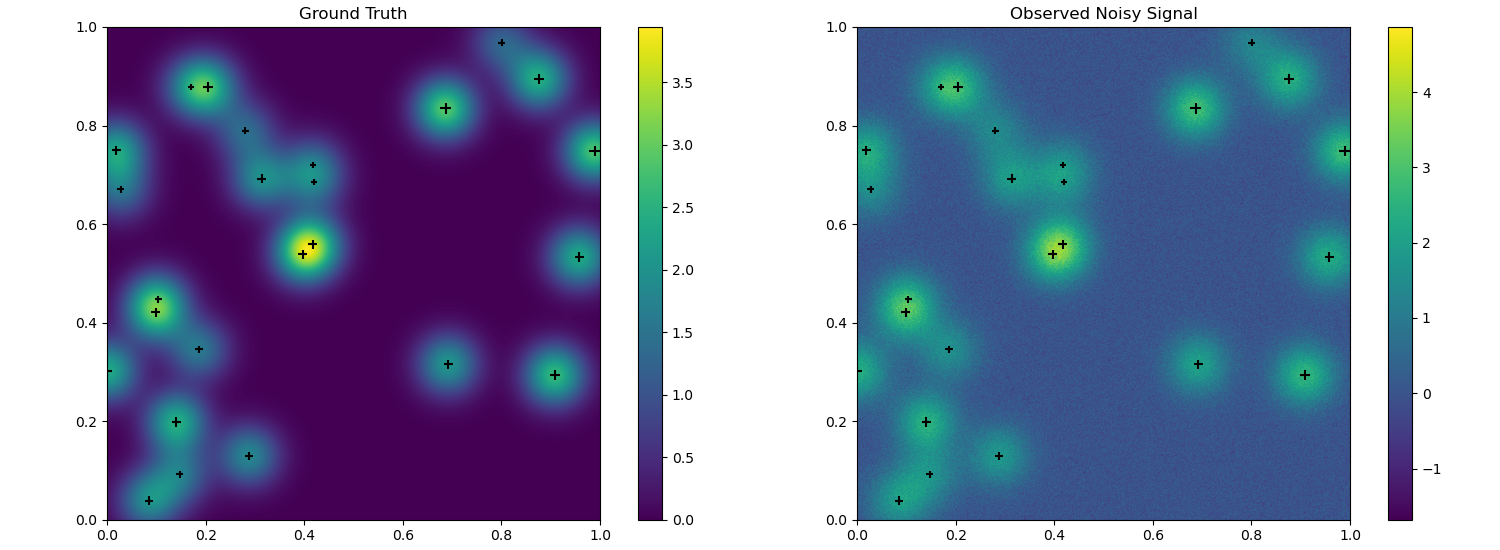
\includegraphics[width=1.2\linewidth]{gt_2d.png}
\caption{Ground truth $\Phi m$ and the noisy measurements $y$. Simulated signal in the case of SMLM.}
\label{fig:gt_2d}
\end{figure}


In SMLM, the Gaussian kernel (also called PSF) is fixed so the FWHM value is fixed in our experiments. The number of measurements and quality of the reconstruction depends only on the definition of the microscope, microscope with a better definition leads to better reconstructions. We show 2 cases, low definition with a pixel size of FWHM/3 and a high definition with a pixel size of FWHM/9. In Figure \ref{fig:gt_2d}, we plot the ground truth $\Phi m$ and the noisy measurements $y$ of a simulates random signal $m$. We reconstruct this signal $m$ with measurements $y$ using both PFW and SFW. The reconstruction with low definition is shown in Figure \ref{fig:PFWvsSFW_2d} and with high definition in Figure \ref{fig:PFWvsSFW_2d2}.\\



The convolved signal is very similarly to the ground truth showing that the solution is consistent with the measurements. In both cases the solution is pretty satisfying and very similar between both algorithms. In 2D, PFW is still less spare compare the SFW and a merge post-possessing step is harder to use, choosing the merging distance seems particularly challenging. To use PFW in practice, we may need to find a solution to this problem. For spikes that are clustered too closely together, the algorithm will reconstruct one spike in the middle, for example at location (0.4, 0.55) in Figure \ref{fig:sfw_2d}. Such cases happen because the Gaussian kernel is too large. With PFW, in some case (e.g. location (0.4, 0.55)), we can reconstruct a better solution with 2 spikes, but in practice it remains impossible to know if the original signal has one or more spikes. Lastly, it is evident that high definition reconstruction has more accurate reconstruction of the spikes, even though it still can not distinguish two spikes that are too close.





\begin{figure}
\centering
\begin{subfigure}[b]{1\textwidth}
   \hspace*{1cm}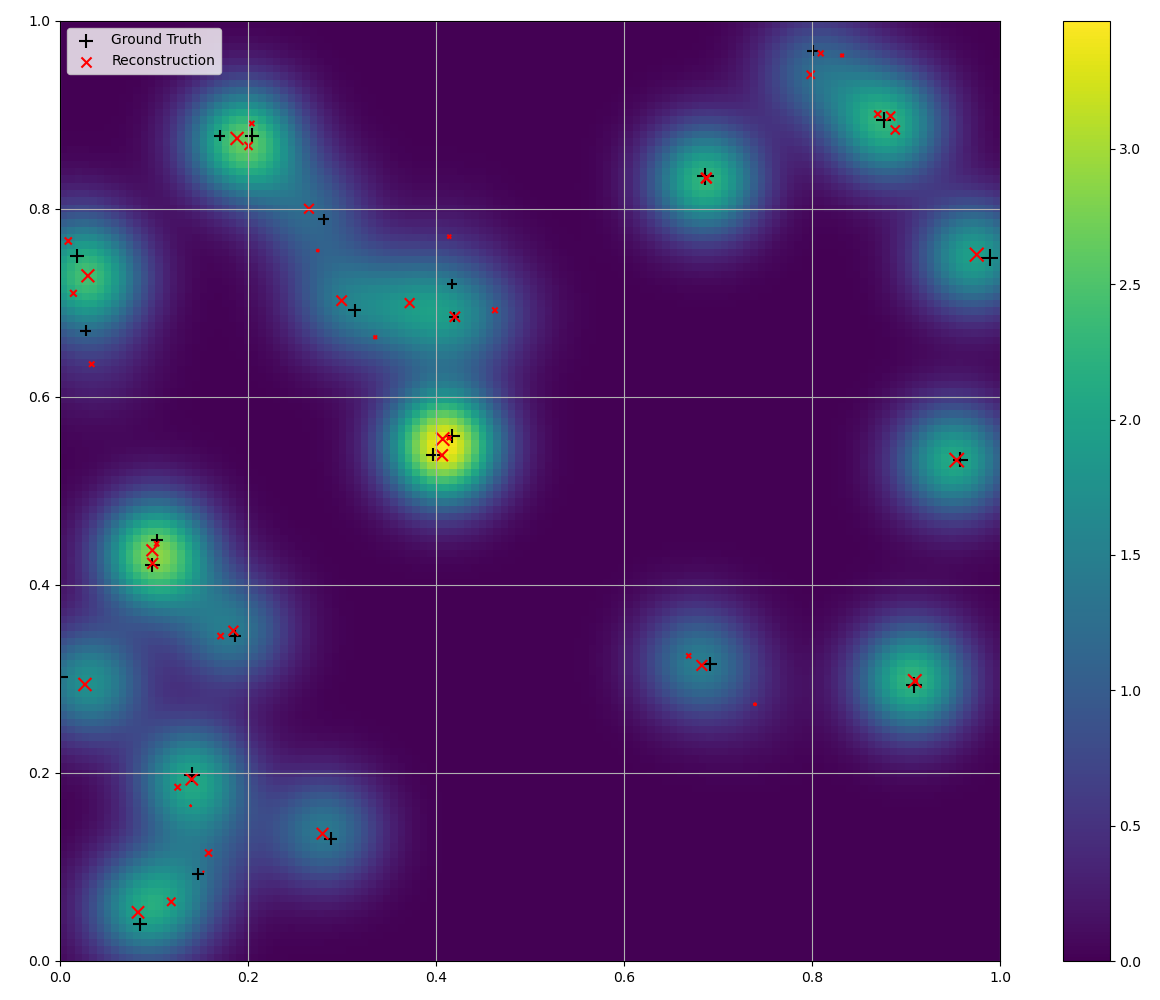
\includegraphics[width=0.8\linewidth]{pfw_2d.png}
   \caption{Reconstruction using PFW}
   \label{fig:pfw_2d} 
\end{subfigure}

\begin{subfigure}[b]{1\textwidth}
   \hspace*{1cm}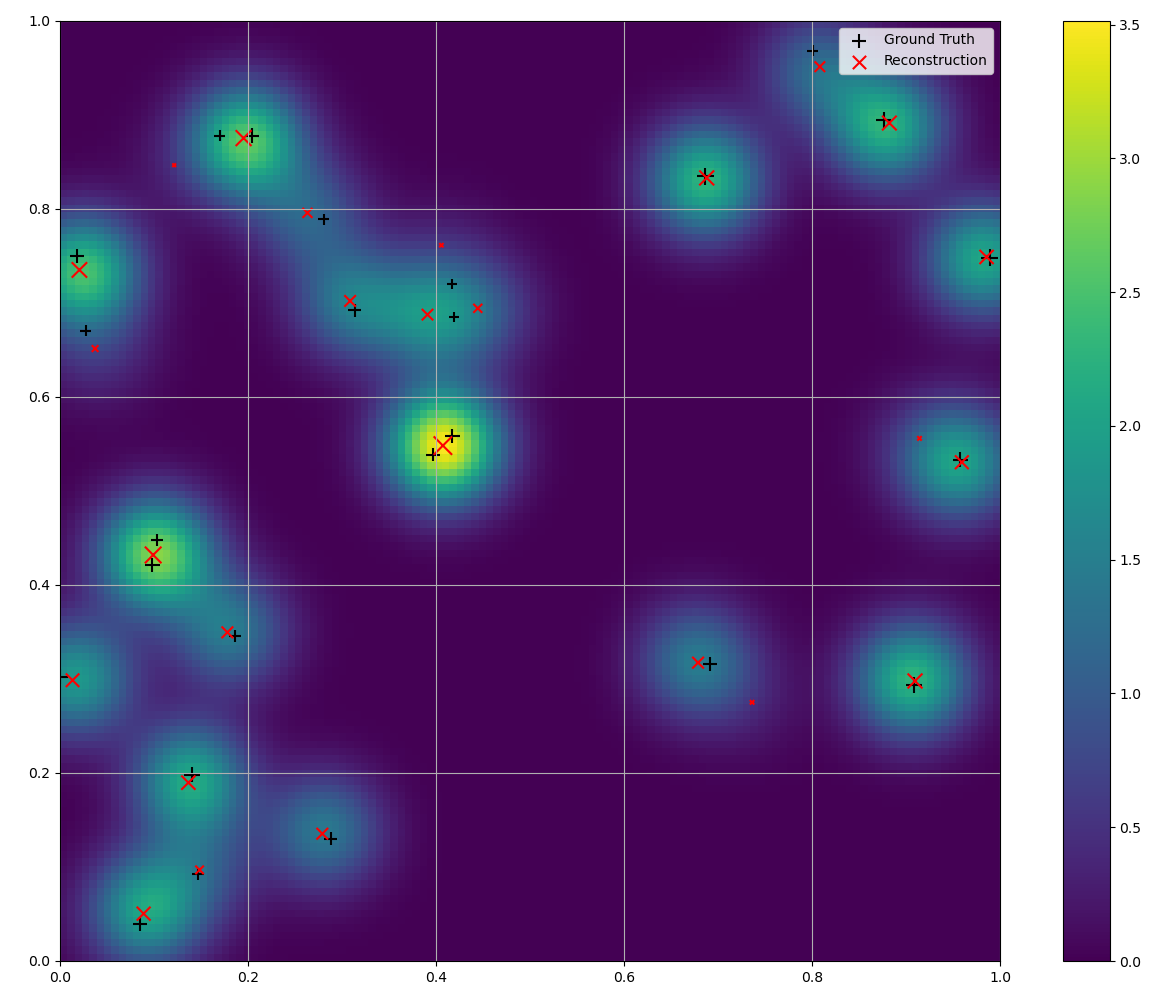
\includegraphics[width=0.8\linewidth]{sfw_2d.png}
   \caption{Reconstruction using SFW}
   \label{fig:sfw_2d}
\end{subfigure}

\caption{Low definition reconstruction.}
\label{fig:PFWvsSFW_2d}
\end{figure}

\begin{figure}
\centering
\begin{subfigure}[b]{1\textwidth}
   \hspace*{1cm}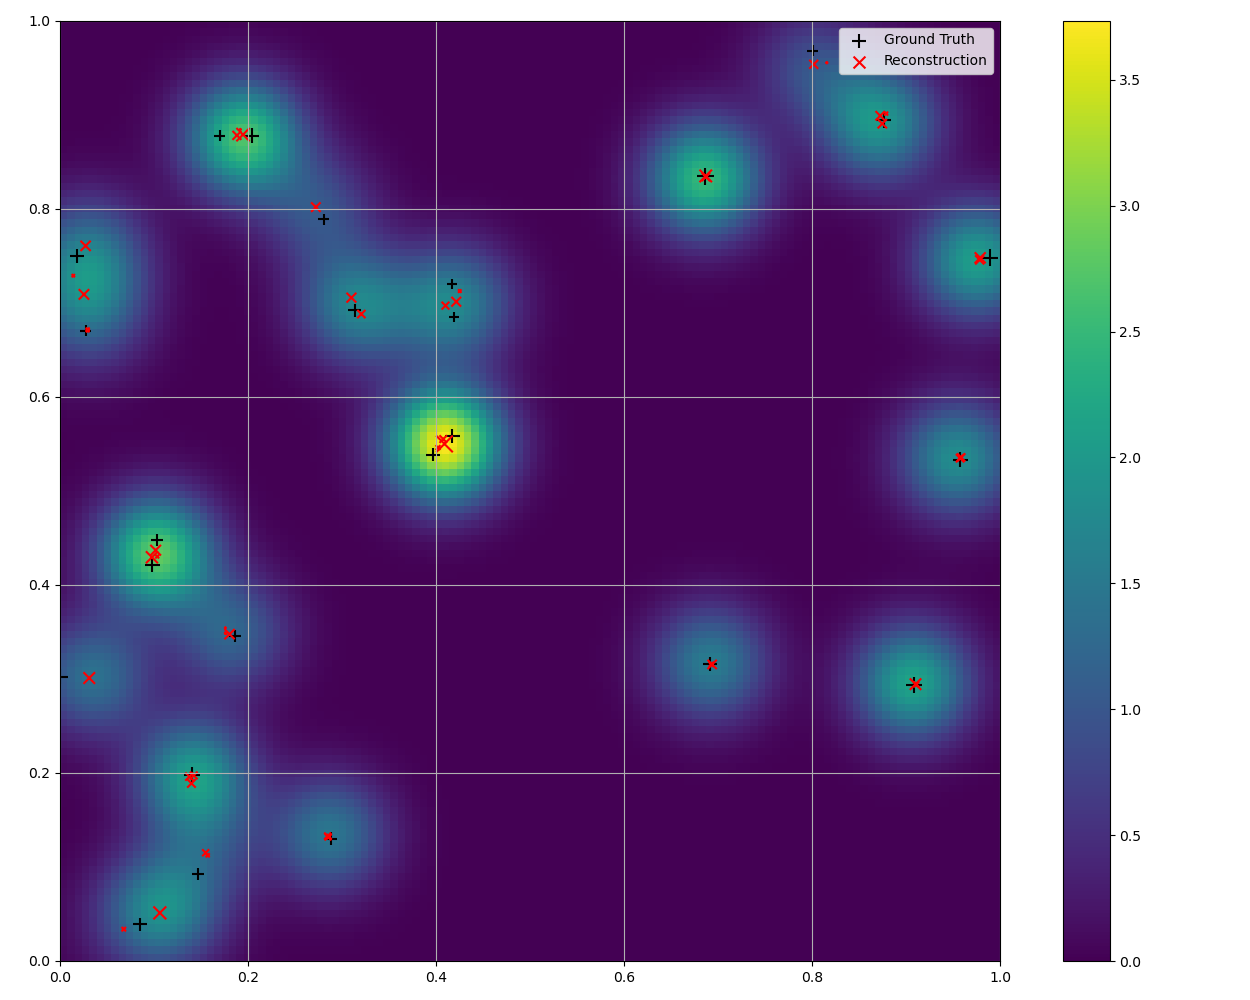
\includegraphics[width=0.8\linewidth]{pfw_2d_2.png}
   \caption{Reconstruction using PFW}
   \label{fig:pfw_2d2} 
\end{subfigure}

\begin{subfigure}[b]{1\textwidth}
   \hspace*{1cm}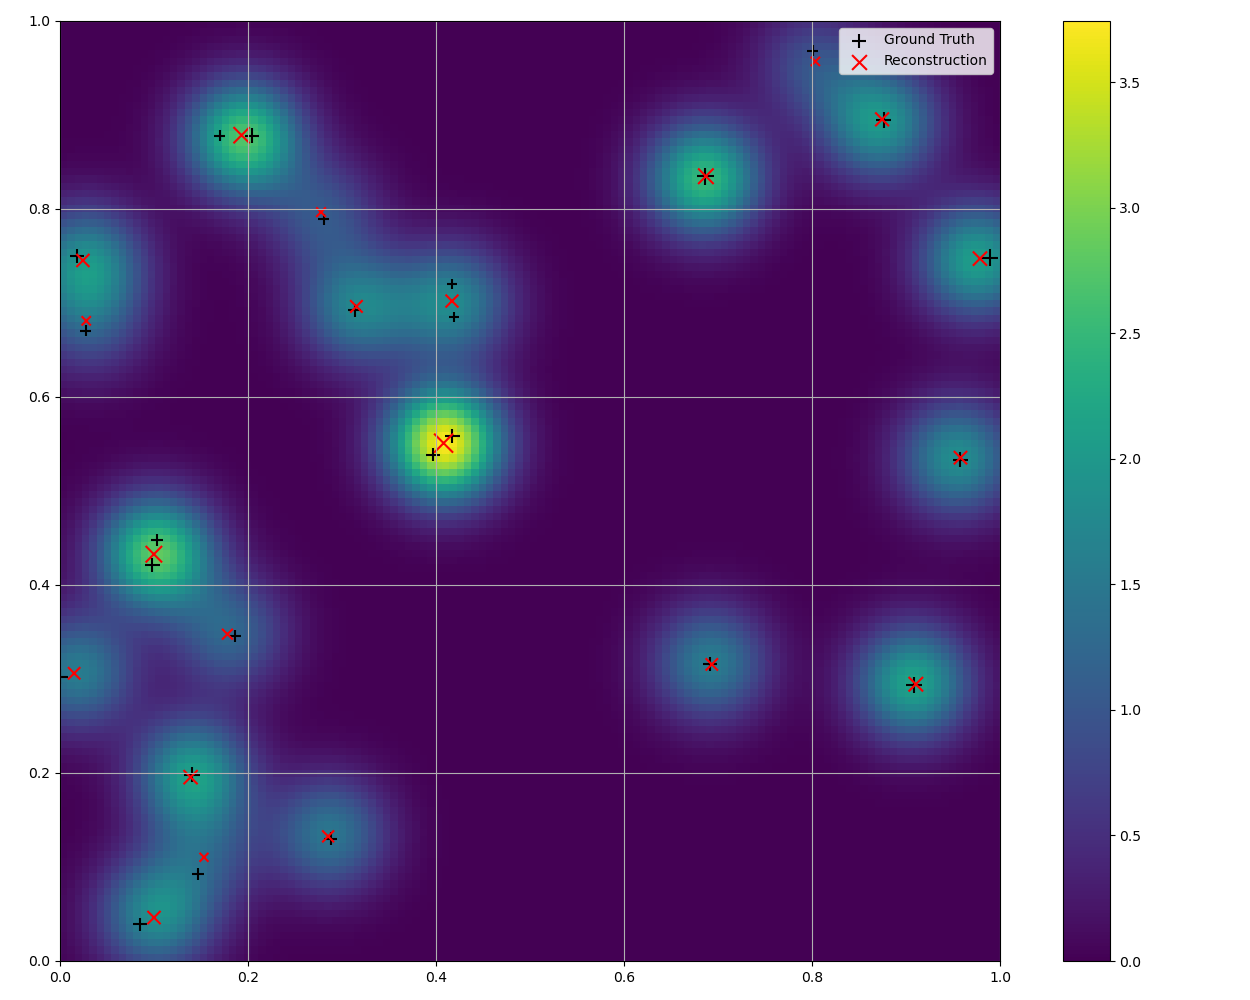
\includegraphics[width=0.8\linewidth]{sfw_2d_2.png}
   \caption{Reconstruction using SFW}
   \label{fig:sfw_2d2}
\end{subfigure}

\caption{High definition reconstruction.}
\label{fig:PFWvsSFW_2d2}
\end{figure}

\newpage
\subsection{2D numeral experiment}
To finish this section on 2D reconstruction, we redo the same experiment as Section \ref{spikes_scaling}, where we reconstruct signals with a varying the number of Diracs using the four algorithms mentions. We show the resulting plot in Figure \ref{fig:n_spikes_2D} and \ref{fig:n_spikes_2D2}. In deconvolution, SFW has a linear scaling with the number of spikes (log curve in a log ax is linear) due to the $N$-step converge property, but it is not the exponential scaling we had above with Fourier measurements, because with convolution we take the same number of measurements no matter the number spikes. PFW has a negligible scaling almost flat showing that the alogrithm is not influenced by the number of spikes to reconstruct. We observe the same critical point at 15 spikes, highlighting whether PFW or SFW is more efficient. Comparing Figure \ref{fig:n_spikes_2D2} with Figure \ref{fig:n_spikes2}, the candidates search step is much more expensive in 2D showing the main bottleneck to higher dimensional reconstructions. We draw similarity conclusion to the 1D case for the variable computation of the PFW's correction step and the bad scaling of the sliding step.


\begin{figure}
\centering
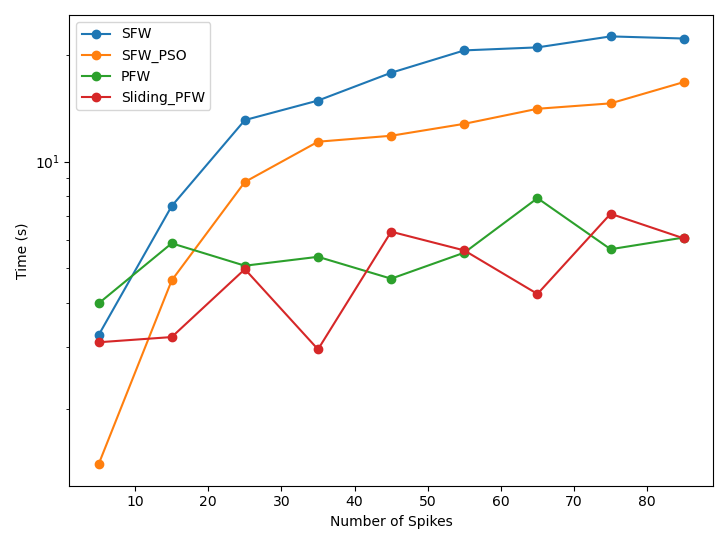
\includegraphics[width=1\linewidth]{n_spikes_2D.png}
\caption{Time in seconds to run for the four algorithms benchmarked with a varying number Diracs to reconstruct.}
\label{fig:n_spikes_2D}
\end{figure}

\begin{figure}
\centering
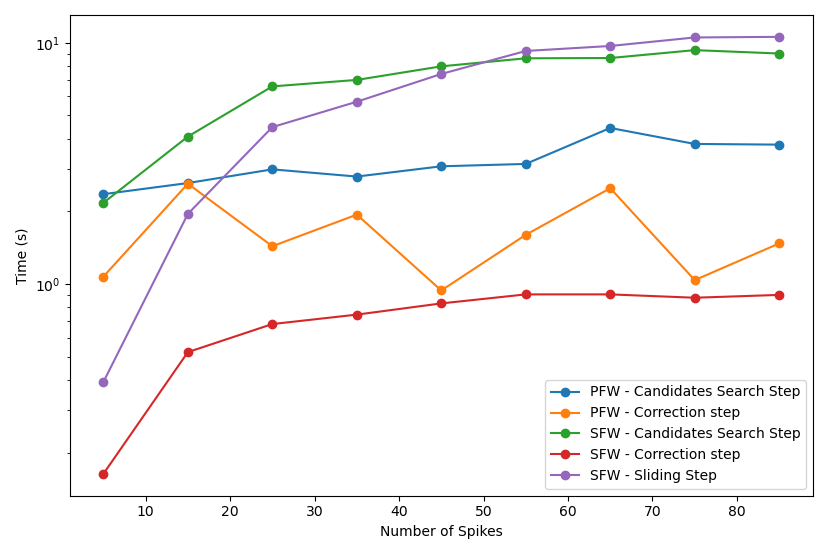
\includegraphics[width=1\linewidth]{n_spikes_2D_2.png}
\caption{Same results as Table \ref{fig:n_spikes_2D}, split into the 3-steps (Candidates Search, Correction and Sliding) for PFW and SFW.}
\label{fig:n_spikes_2D2}
\end{figure}

\chapter{Conclusion}

In this work, we introduced a polyatomic Frank-Wolfe algorithm as an innovative solution to the BLASSO optimization problem, providing advancements in grid-free sparse spikes reconstruction. The proposed method leverages polyatomic updates to enhance the exploration of the solution space and accelerate convergence. Our study highlights the advantages, limitations, and unique characteristics of PFW. Through numerical experiments, we demonstrated the algorithm's superior efficiency and scalability compared to state-of-the-art methods such as the Sliding Frank-Wolfe algorithm. The results demonstrate that PFW offers significant computational advantages when reconstructing signals with numerous Diracs. \\

Key contributions include the development and research of candidates selection strategies. Our work showed that polyatomic updates, while computationally more intensive at each iteration, drastically reduce the total number of iterations required and can be a great improvement to any Frank-Wolfe-based algorithm. Furthermore, the addition of a post-processing merging step provides a sparse solution that closely aligns with the SFW results without incurring the sliding step's computational overhead. Applications to 1D and 2D signal reconstructions highlighted the algorithm's practical performances in both Fourier measurements and deconvolution. These findings underline the potential of the polyatomic Frank-Wolfe approach.\\

Looking forward, future work could explore alternative techniques for sparsification, enhancing the candidates selection in particular improve the idea of smoothing the dual certificate or alternative mathematical frameworks to enhance PFW’s efficiency. By advancing these directions, the polyatomic Frank-Wolfe algorithm could become a cornerstone methodology for grid-free sparse recovery.




\addcontentsline{toc}{chapter}{Bibliography}
\bibliography{refs.bib}{}
\bibliographystyle{plain}

\end{document}
